\documentclass[11pt]{report}
\usepackage{listings}
\usepackage{graphicx}
\usepackage{amsmath}
\usepackage{enumitem}
\usepackage{makecell}
\usepackage[T1]{fontenc} % Use 8-bit encoding that has 256 glyphs
%\usepackage{fourier} % Use the Adobe Utopia font for the document - comment this line to return to the LaTeX default
\usepackage{hyperref}
\usepackage[english]{babel} % English language/hyphenation
%\usepackage{amsmath,amsfonts,amsthm} % Math packages
\usepackage{placeins} % keeps floats (e.g. Tables) within "\FloatBarrier" boundaries
\usepackage{float}
\usepackage{mathptmx}
\usepackage{sectsty} % Allows customizing section commands
\allsectionsfont{\normalfont} % Make all sections centered, the default font and small caps \sectionfont{\fontsize{12}{15}\selectfont}
\usepackage{gensymb}
\usepackage{fancyhdr} % Custom headers and footers
\pagestyle{fancyplain} % Makes all pages in the document conform to the custom headers and footers
\fancyhead{} % No page header - if you want one, create it in the same way as the footers below
\fancyfoot[L]{} % Empty left footer
\fancyfoot[C]{} % Empty center footer
\fancyfoot[R]{\thepage} % Page numbering for right footer
\renewcommand{\headrulewidth}{0pt} % Remove header underlines
\renewcommand{\footrulewidth}{0pt} % Remove footer underlines
\setlength{\headheight}{13.6pt} % Customize the height of the header
\usepackage{cite}
\usepackage{chngcntr}
\setcounter{equation}{0}

\makeatother

%usepackage[backend=bibtex,style=verbose-trad2]{biblatex}

%\bibliography{grasp_bibtex_papers}
\numberwithin{equation}{section} % Number equations within sections (i.e. 1.1, 1.2, 2.1, 2.2 instead of 1, 2, 3, 4)
%\numberwithin{figure}{section} % Number figures within sections (i.e. 1.1, 1.2, 2.1, 2.2 instead of 1, 2, 3, 4)
%\numberwithin{table}{section} % Number tables within sections (i.e. 1.1, 1.2, 2.1, 2.2 instead of 1, 2, 3, 4)
\setlength\parindent{0pt} % Removes all indentation from paragraphs - comment this line for an assignment with lots of text
\usepackage{preview}
\usepackage{gantt}
%----------------------------------------------------------------------------------------
%	TITLE SECTION
%----------------------------------------------------------------------------------------

%\newcommand{\horrule}[1]{\rule{\linewidth}{#1}} % Create horizontal rule command with 1 argument of height

\title{
\normalfont \huge
\textsc{AI-assisted short answer grading: comprehensive classification and evaluation of the existing state of the art techniques \\Proposal for RnD Project
} % Your university, school and/or department name(s)
%\horrule{0.5pt} \\[0.4cm] % Thin top horizontal rule
%\normalfont Probabilistic Assignment 4 \\ % The assignment title
%\horrule{2pt} \\[0.5cm] % Thick bottom horizontal rule
}
\usepackage{amsmath,amsthm,amssymb}
\author{Student: \\Evgeniya Ovchinnikova\\
\\Supervised by:
\\Prof. Dr. Paul Ploeger
\\M.Sc. Deebul Nair } % Your name

\date{\normalsize 16 April, 2018} % Today's date or a custom date


\begin{document}

\counterwithout{equation}{chapter}
\counterwithout{equation}{section}
\counterwithout{equation}{subsection}
\maketitle % Print the title
\thispagestyle{empty}
%----------------------------------------------------------------------------------------
%With This template you can add code, image and sections.
%----------------------------------------------------------------------------------------------
\newpage
\pagenumbering{arabic}
\chapter{\textbf{Introduction} }

The process of teaching is very challenging and takes considerable time and effort. In many areas, especially computer science, it requires keeping the curriculum and assignments up to date and relevant. Personal communication with students and giving feedback on tests and homework is also essential as well as time-consuming. These activities are the most visible to students, but there are many more things a teacher or professor must do, such as paperwork, organizational issues, to name just a few. For this reason it is important to optimize the time dedicated to each different aspect of work. Keeping course content relevant as well as personal communication cannot be easily outsourced, but grading tests and assignments is usually straightforward enough and does not require a professor's expertise. Students often make similar mistakes, making the task well-suited for automation using machine learned models. This clearly shows that it is an ideal task to be automated.\\

Assignments and test answers include different aspects, such as text, pictures and programming code. In this work we focus on the text. There are several main text answer types: "fill the gap", short as well as long answer essays ~\cite{Hasanah}. The first type does not represent a complex problem because there would normally be only one possible answer and the only challenges that one can face here are handwriting recognition, if the test was not on a computer; or spelling correction, if the incorrectly spelled answers can be accepted. Two other types are more challenging from the text analysis point of view. Automated essay scoring (AES) focuses on evaluating texts longer than one paragraph, whereas automated short answer grading (ASAG) concentrates on answers consisting of a small number of sentences ~\cite{Hasanah}. The other important difference is that ASAG only concerns the with the meaning of the answer, while for AES the writing style is also very important ~\cite{Burrows}. \\

AES is a rather complex task. Some massive open online courses (MOOC), such as those offered by EdX, MIT and Harvard's non-profit organization HarvardX, and organizations like ETS have already started using the automated essay grading systems  ~\cite{Balfour}, ~\cite{aesOverview}. This is a logical step, since most of the online courses are either free or very cheap in comparison to the ones in real universities and institutes and it is impossible to find many teachers who are willing to work for free. They use an algorithm developed by one of the contestants ~\cite{vikGit} of "The Hewlett Foundation: Automated Essay Scoring" competition on Kaggle ~\cite{HewlettKaggle} and an EASE library ~\cite{edxGit}, which can be used for machine learning text classification. Although AES has been received rather positively ~\cite{aesOverview},~\cite{Shermis},~\cite{Alikaniotis}, there are still many people who have strong doubts about the feasibility of automated essay grading. Many people, including even Noam Chomsky, have signed a petition "Professionals Against Machine Scoring Of Student Essays In High-Stakes Assessment" ~\cite{petition}. Moreover, there were a lot of papers criticizing either state of the art AES or its general appropriateness ~\cite{Perelman}, ~\cite{Byrne}, ~\cite{Ramineni}.\\

Good AES research requires a solid computational linguistics background. Moreover, this area is more relevant for the humanities. This research concentrates on developing an AI assistant for grading assessments and exams in the fields of computer science, electrical engineering, physics and other technical disciplines. Here the answers are usually shorter and more concrete. Furthermore, stylistics and spelling are not of interest, but that depends on the individual professor. Therefore this work focuses on ASAG. This task is viable and the solution should be helpful for both professors and students. It can allow professors more time for other teaching activities and provide students with faster and less biased feedback on their work.

 
\chapter{\textbf{State of the art}}

\section{\textbf{Natural language processing}}

\subsection{Natural language processing development}

This work focuses on ASAG that is a very narrow subfield of natural language processing (NLP). Therefore it is important to consider what actually is NLP first.\\

NLP is an very important research area that developed from the simple algorithms those could be performed on punch cards to huge sufisticated and heavy calculations those are performed by compamies like Google and Facebook now ~\cite{Cambria}. NLP is based on many other subject areas, such as linguistics, mathematics, computer science, artificial intelligence, robotics, and psychology. It can be applied in such areas as machine translation, summary generation, simplification of the texts, multilingual and cross-language information retrieval, diagnosing, chat-bots development, etc. ~\cite{Chowdhury}. The common idea among these tasks is that the computer must truely understand the language, the meaning of the phrases, sentences and whole texts. However, we cannot just tell the machine to "understand", its "understanding" must be formalized. This formalization is the subject of NLP. In a broader sense NLP task includes all levels of language processing and understanding: acoustic (speech recognition), analytical (syntactics and semantics), contextectual (anaphora, inference of referents, etc.), inferential (detection of inferences and implicatures), planning (sense, text and speech generation). Otherwise NLP can be narrowed mainly to analytical part, i.e. be considered as a set of techniques and methods for grammatical structure extraction and analysis for text understanding  ~\cite{Steedman}. Current work is not interested in such aspects of NLP as speech recognition and generation or in detailed research on grammars, the most interesting NLP aspect is an information extraction -- "subset of knowledge discovery and data mining that aims to extract useful bits of textual information from natural language texts" ~\cite{Chowdhury}.
However, text generation can be another useful tool for teachers who are interested in automated generation of examination questions, and speech recognition can be interesting for oral exams aytomation in the future. Therefore we will briefly consider all seven stages that may include a task of NLP ~\cite{Chowdhury}, ~\cite{Saad}:
\begin{itemize}
\item Phonetics
\item Morphology
\item Lexis 
\item Syntax
\item Semantics
\item Discourse
\item Pragmatics
\end{itemize}
 
Phonetics doesn't extract any meaning of the words, it is only focused on pronunciation. At this level an NLP system is focused more on a signal-processing than a linguistic part, though linguistic tools can be helpful in disambiguation of badly-parsed text.\\

Morphology is the most low-level stage of text processing: it considers the structure of the words, words' parts and how these parts influence the meaning of the words. For example, if "s" is added to a noun that would be a plurality morpheme and "s" added to a verb would indicate that it is the verb used in combination with a noun or pronoun that describes a third person.\\

Lexis considers the level of the words and parts of speech. Unlike in morphology at this level the meaning of the separate words is extracted regardless of their forms, e.g. the words "mouse", "mice" and "mouse's" can be the same lexical entity.\\

Syntax is the third level that considers the grammar of the language. It breaks the sentence into separate members of a sentence, i.e. subject (nominative), attribute (verb), case put after (object), etc., and reorganizes the data in such a way that can be analyzed by computer. This analysis includes grammar and parsing ~\cite{Saad}.\\

Semantic is a higher level analysis that considers extraction of meaning of words and sentences. \\

Discourse the highest level information extraction that considers the information extraction of text parts larger than a sentence, or the whole text. It deals with the whole structure of the document. The knowledge from this level can be very helpful for text summarization. \\

Pragmatics is the outer level of information extraction that includes the knowledge about the world, which is not contained in the document. It consists of two stages: finding ambiguities and disambiguation. The are following types of ambiguities: one-word long lexical (homonym) and referential ("it", "he", etc.), several-words long syntactic, sentence-long semantic, local (context requiring, which is usually a great issue for translation). Disambiguation includes the following methods: probabilistic (simple choice of the most common meaning of the word, optionally -- most possible in the subject field of this text), conditional probability (choice of the most common meaning of the word in the subject field of this text), context (most probable meaning of this word when it is surrounded by certain words or grammatical structure), world models (disambiguation by usage of world states)  ~\cite{Saad}. The conditional probability can be especially important for this work, because the tests are subject-specific and would normally use only one meaning of the certain word. For example, the word "operation" in a computer science exam will with almost 100\% probability not mean mean "surgery" . \\

History and prediction of integration of the methods mentioned above into NLP over is shown in Fig.\ref{fig:NLPLevels}. One can clearly see how the computers could grasp gradually more general meaning of the text. From understanding of single words to acquiring the meaning of whole sentences and paragraphs. Such differences are always easy to see in machine translation. One can compare the translation given by Google-translator (\url{translate.google.com}) that uses the bleeding-edge NLP-methods and PROMT (\url{http://www.online-translator.com/}) that translates almost word by word. The original sentence was takes from the beginning of "Faust" by Johann Wolfgang Von Goethe: "Ihr n{\"a}hert sich wieder, schwankende Gestalten, Die vor sich selbst ist der Tr{\"u}ben Blick gezeigt.". The translation by Google is "You approach again, swaying figures, who in front of themselves is shown the murky gaze.", by PROMT -- "You approach again, fluctuating shapes, early to yourselves once the murky look shown.". PROMT couldn't even detect the German structure of the sentence and just put the English words in the initial order. Google translation is not perfect, but it is clear that it translates the whole sentence and not only the separate words. However, even a relatively good automated translator has problems with textual ambiguity and especially stylistics and it will take some time before it is able to translate the literature like human translators: "Again ye come, ye hovering Forms! I find ye, As early to my clouded sight ye shone!" ~\cite{Faust}.\\ 

\begin{figure}[h!]
  \centering
  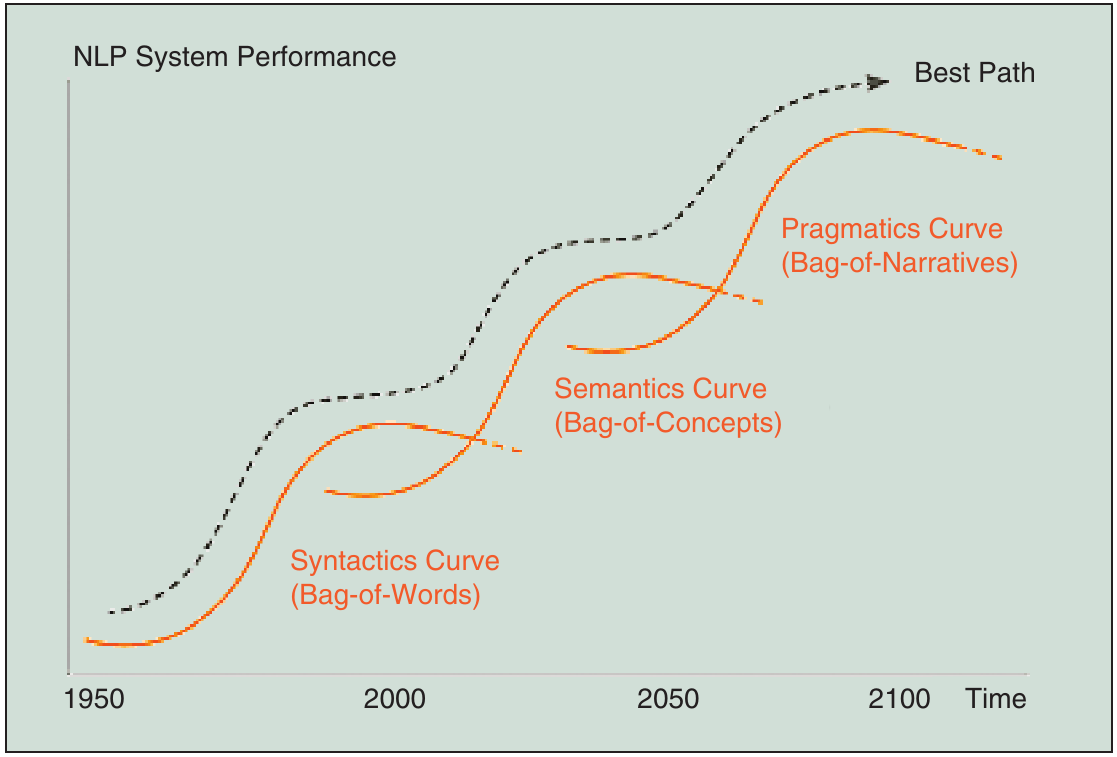
\includegraphics[width=0.8\textwidth]{img/NLPLevels}
    \caption{ Envisioned evolution of NLP research through three different eras or curves ~\cite{Cambria} }\label{fig:NLPLevels}
\end{figure}

Though semantic approach is slowly starting being used more commonly, syntactic approach is still used more often. That is why it is important to mention the main methods used there ~\cite{Cambria}:

\begin{itemize}
\item Keyword Spotting -- unambiguous buzzwords detection. It is used in the following systems:
\begin{itemize}
\item Ortony's Affective Lexicon -- for words categorization;
\item PageRank -- Google's page ranking algorithm;
\item TextRank -- graph-based ranking model for text processing.
\end{itemize}  
\item Lexical Affinity -- allows to detect not only unambiguous words, but also assign words to a certain group with a given probability based on a certain text corpora, e.g. "operation" can be medical with 40\%, computational with 30\% and military -- with 30\%. The problem of this approach is that it can easily be overfitted and work only for one area on which word probabilities it was trained.
\item Statistical NLP includes the following machine learning algorithms:
\begin{itemize}
\item maximum-likelihood
\item expectation maximization
\item conditional random fields
\item support vector machines 
\end{itemize}
The method allows to learn by training on a large text corpora the valence of the buzzwords, while also taking into consideration punctuation and how often certain words occur together. The problem of this method is semantic weakness: it's too focused on the buzzwords and cannot work efficiently enough with other words, therefore it requires a very large amount of text to train.
\end{itemize}

Semantic or concept-based level is fundamentally different: it is focused on the meaning of sentences as a whole and not on spotting of separate buzzwords, learning the concepts and not the words. One can distinguish the following concept-based NLP approaches ~\cite{Cambria}:
\begin{itemize}
\item internal knowledge-based techniques (endogenous) -- uses only information from a given document. It integrates machine learning in order to conduct lexical-semantic analysis of a large amount of textual information to extract concepts. The following machine learning methods are used:  
\begin{itemize}
\item latent semantic analysis -- vector documents in a terms space;
\item latent Dirichlet allocation -- assigning terms to topics;
\item genetic algorithms -- probabilistic pseudo-stochastic search. 
\end{itemize}
\item external knowledge-based techniques (endogenous) -- used external information about the world. There are two main categories of those:
\begin{itemize}
\item taxonomic or ontology-based approaches are usually concerned about the "isA" relations between objects (e.g. "Albert Einstein") and concepts (e.g. "physicist"). The problems of this approach are bad scalability and that the representation of knowledge is too strictly-defined and typical. It overdefines the object and considers only its "proper" usage, for example an idea of a "key" can be related to a "picklock" or a "wireless keycard", as they are used to open a door, but not to other possible usages of the key, as a sort of weapon or a beer opener.
\item noetic or semantic knowledge-based include all human brain-based techniques. It focuses on semantic parsing nd linking separate linguistic components creating meaningful constructions. The following machine learning methods are used for this:
\begin{itemize}
\item neural networks
\item deep learning
\item sentic computing 
\end{itemize}
\end{itemize}
\end{itemize}



\subsection{Linguistics and NLP.}


All the concepts mentioned above originate in pure linguistics and it is obvious that NLP area would strongly rely on linguistics. However, it is a hard question, how much NLP should rely on pure linguistics and which modifications should be applied to linguistic methods so they would be efficiently applicable to NLP. Linguistics provides a highly-formalized model of the language. Raskin in ~\cite{Raskin} names the following manifestations and interpretations of linguistic formality:

\begin{itemize}
\item mathematical notation usage
\item mechanical-symbol-manipulaticn-device (MSMD) approach:
\begin{itemize}
\item collecting all information without any filtering and representing it in a mathematical form, e.g. formal grammar
\item creating a number of subsets of linguistic items with common features
\item all the subsets together must cover all the words those were considered
\item it is assumed that a native speaker must be able to differentiate all these items intuitively, without any specific knowledge
\end{itemize}
\end{itemize}

This approach seems formal enough to directly transfer it to a format acceptable for machine text processing without fundamental concept changes. However, it is not that easy and direct application of the method would usually lead to a bad result. One must know certain laws of a correct usage of pure linguistics in application to NLP. It is important to understand that the problem should originate in a target field (NLP), whereas approach and terms can come from the source field (linguistics). Otherwise it would be impossible to reach the target and use the source efficiently ~\cite{Raskin}. Plainly linguistic problems should not be formulated for NLP-tasks, however, linguistic approaches remain crucially important for NLP ~\cite{Steedman}. The NLP task includes the following ~\cite{Chowdhury}: 
\begin{itemize}
\item thought processes
\item representation and meaning of the language input
\item world knowledge of the program
\end{itemize}

Table \ref{NLPvsL} shows the main differences between NLP and pure linguistics those help to understand how to use linguistics for the task of NLP.\\

\subsection{NLP and ASAG.}

//add the methods I'm going to use

\begin{table}[]
\centering
\caption{Difference between linguistics and NLP ~\cite{Raskin}}
\label{NLPvsL}
\begin{tabular}{|l|l|}
\hline
 \makecell{Linguistics} & \makecell{NLP} \\ \hline
 \makecell{research on usage of sounds\\and its meaning for the language} & \makecell{ parsing spoken language to a written\\form for information extraction} \\ \hline
  \makecell{structuring the meaning of the text} &  \makecell{understanding the meaning of the text}  \\ \hline
  \makecell{categorizing different linguistic\\structure levels} &  \makecell{making a text source-independent by \\ extracting all relevant information}\\ \hline
 \makecell{separating linguistics and\\encyclopedic information} & \makecell{using encyclopedic information in \\combination with linguistic approaches} \\ \hline
 \makecell{formal (set of rules) representation\\of the result} & \makecell{making the information practically\\ accessible} \\ \hline
 \makecell{\textbf {language in general}} &  \makecell{\textbf{narrow part of the language}}  \\ \hline
\end{tabular}
\end{table}


The last point is especially important for the current work. It shows that it is common to use a very limited subset of the words existing in a language for NLP in general. It is also the case for our task, because each exam is dedicated to a certain subject with its own lexicon. Moreover, the formal nature of examinations allows to discard all informal and colloquial words. A student is normally not allowed to use sentences with slang and colloquial terminology similar to the following examples: "Yukio Mishima was a totally screwed wacko and a bent, but it is not the only reason why we all like him", "You should never forget to shiled the qubits properly, otherwise your experiment will be absolutely screwed". In the set of words those a formal exam would allow, "screw" as a verb should only mean "an act of turning a screw or other object having a thread" (\url{https://www.google.de/search?q=Dictionary}) and "bent" would only be a past or an adjective form of "bend".  That is why it is not efficient to try using general linguistic methods, though they are supported by the whole power of the language. Instead it makes sense to focus on NLP-methods those would allow to concentrate on specific subject-specific words. Raskin names the following advantages of the sublexicons ~\cite{Raskin}:

\begin{itemize}
\item on average it contains several hundred words instead of 500 000  
\item ambiguity is drastically reduced due to the reduced number of meaning homonyms (see examples above)
\item only a very limited extralinguistic knowledge of the world is needed
\end{itemize}

However, it is important not to forget that this approach can overlimit the lexicon and make the approach not extrapolatable enough. For example, if one develops an exam in the area of physics, he or she might want to reduce the set in such a way that a word "induction" would mean only "electromagnetic or magnetic induction" and it cannot mean "mathematical induction". It doesn't make much sense though, because adding this sense to such word is not very costly and in general it is possible to use a similar set of words for mathematics and physics, which would allow to have more train exam samples. Moreover, this approach is dangerous because even in one area it is not always possible to foresee all possible vocabulary that will be used.


\section{\textbf{Automated grading}}

Research in natural language processing (NLP) started in 1950. The following topics were and still are the main focus of NLP researchers: automatic translation, information retrieval, summarizing of texts, question answering, information extraction and topic modeling  ~\cite{Cambria}. Sixteen years later, in 1966, the first work on automated grading was published ~\cite{Page}. That first work was dedicated to essay grading and it laid a foundation to a large field that now includes automated essay and short answer grading. The main differences are listed in Table \ref{ASAGvsAES} ~\cite{Burrows}, ~\cite{Hasanah}, ~\cite{Ziai}. This section is focused on analysis of current state of the art in these two areas.

\begin{table}[h!]
\centering
\caption{ASAG vs AES}
\label{ASAGvsAES}
\begin{tabular}{|l|l|l|}
\hline
 & Short answer &  Essay \\ \hline
 Length & $\leq$ one paragraph & $>$ one paragraph  \\ \hline
 Evaluation criterion & Content &  Style, content \\ \hline
 Openness & Closed &  Open \\ \hline
 Question format & Formulated according to strict rules & Can be general \\ \hline
 Correct answer & Exists & Doesn't exist \\ \hline
\end{tabular}
\end{table}



\subsection{AES}

In recent years massive tests, such as language proficiency exams (TOEFL, IELTS, TestDaF, DELF, etc.) or MOOC assessments, are becoming increasingly popular. All language tests and many MOOC assignments contain parts where the students have to either summarize a given text or write his/her own text or essay. Scoring these long text is a huge task that requires tremendous amount of human power. Language tests are rather expensive, thereby it is possible to find enough people to grade them. The idea of MOOCs, however, is to make the courses from the best universities affordable for people and that is why it is why scoring is a big issue in this case. It is possible to automate multiple-choice tests, but the quality of such check of knowledge is very low. Therefore, it was essential to automate free text grading as well. Moreover, it is still important for the language tests, because the autograding would allow to give a faster and less biased response.\\

Both, automated and human essay grading, have several important issues those must be faced -- see table \ref{Issues} ~\cite{Blood}. Therefore, starting the automated grading was a long process, but now it is rapidly developing. \\


\begin{table}[]
\centering
\caption{Issues of automated and human grading}
\label{Issues}
\begin{tabular}{|l|l|}
\hline
 \makecell{Automated grading} & \makecell{Human grading} \\ \hline
 \makecell{It is hard to define an impersonal criterion\\ for text style quality: many long-text\\ tasks require not only correctness of content,\\ but also a good writing style and/or usage\\ of certain constructions. In tasks\\ like "Describe a graph", which a participant has\\ to do on TestDaF and IELTS, one should only\\ use certain constructions and be relevant, however,\\ in essay part the style, which\\ can be estimated differently even by\\ human examiners, plays an important role. } & \makecell{Human graders must be\\ specifically trained, which requires\\ a massive amount of time and money.} \\ \hline
 \makecell{Though it is not intentionally malicious,\\ autograder can still be biased. For example,\\ if students with similar writing style \\usually deliver works of bad quality,\\ the system can overlearn in such a way that\\ it would rate badly even good works of\\ similar style.} & \makecell{ Human graders are biased more likely\\than a machine. Therefore\\test organizations try to avoid\\such bias by a complex\\ cross-validation, testing and\\ changing the assignments in such a\\way that the possible bias is\\ reduced, which requires a\\lot of time and\\financial resources. } \\ \hline
  \makecell{Usage of AES may cause negative reaction of \\examenees.} &  \makecell{The high costs reduce the number of\\people who can afford to take an exam.}  \\ \hline
    \makecell{AES might have problems with gibberish\\detection.} &  \makecell{"Human factor" like sickness\\ or any other problems\\of the grader may cause\\a significant increase of grading\\time or decrease of grading\\ quality. }  \\ \hline
\end{tabular}
\end{table}


The first multiple-choice grader was developed in 1938, whereas the first idea of the free text grader appeared only in 1960's in a work of Ellis Page ~\cite{Blood}. The system was called Project Essay Grade (\textbf{PEG}). His approach was based on usage of proxes and trins -- the variables recognizable by a machine and a human graders accordingly, e.g. a number of words could be a prox and elaboration -- a trin. The method was based on training the multiple-regression algorithm to grade like humans in a train set, not on the analysis of the text itself. The main features of the texts were the number of words and word length, which allowed to reach a correlation of 0.71 (0.77 in the later releases) with the human graders. The correlation between the machine grading and human graders was shown to be higher than the correlation between different human garders ~\cite{Blood}. This grader, however, was very vulnarable to "gibberish" texts, i.e. the ones containing completely senseless words like "bzhykhlvyazsk" or "bdvfngjvsbcdhkuhlhdsskmlklewnmx" ~\cite{Shermis}. The words are long and the text can be as long as the writer please, however, it is not a real essay and by a human teacher it would be graded with zero points. The 0.77 correlation was obtained in absence of such important test cases. It shows a great importance of proper dataset that would cover most of the possible test cases. \\

Almost 40 years after the development of Page's approach of using the human graders' scores instead of a real understanding of text by computer as a main training criterion was of current interest. For example, \textbf{E-Rater} developed by ETS (the organization that conducts TOEFL and GRE) in 1990's operated in the similar way and also used multiple-regression method combined, however, with NLP, which allowed to include grammatical accuracy. The latest (2006) version had an additional feature that took into account word overlap between test and train essays, which was considered rather advanced, because it allowed to reduce importance of essay length, which essentially should not be an indicator of quality. This system is now used in GRE, TOEFL and several other ETS's tests. Correlation with human scores is very high -- 0.97, again higher than between human raters ~\cite{Blood}. However, there is still a lot of criticism. For example, it was shown that examnee can submit a text -- so-called "word salad" -- that is long enough, contains all right and long words and constructions, but still doesn't make any sense, and the system will still grade it highly, for it meets all the needed requirements ~\cite{Hearst}. Another point voiced by critics is that the system can grade a good and creative essay, which doesn't meet some formal requirements, badly. That is another reason why many people including prominent scientists like Noam Chomsky argue that AES brings no good to the education ~\cite{petition}. It is true, however, such requirements is one of the examples when people expect from machine a way better performance than from humans. A human rater receives a massive amount of written works those must be graded in a short time. Human grading in this case is as formal as machine grading and creativity can be punished by a bad grade as possibly as in case of machine grading. Moreover, human graders are shown to have less unity among each other in their judgements than with machine, as it was shown in experiments with both, PEG and E-Rater ~\cite{Blood}. Individual approach is important, but it is feasible only in small groups. In case of massive courses it is equally formal, no matter if it is an automated or human grading.\\

PEG and E-Rater had the same base idea. A fundamentally new approach was introduced in 1998 by \textbf{Latent Semantic Analysis} (LSA) ~\cite{LSA}. The main difference was that the method started caring about the meaning of the text and not only on breaking it into linguistically non-meaningful features those will be weighted and learned in relation to the human grades. In this method statistical  computations on a large corpus of text are used to extract the contextual meaning of words, which places the method semantic part NLP curve (Fig. \ref{fig:NLPLevels}) ~\cite{LSA}. Moreover, the goal of methods developers was to imitate the way humans obtain and classify knowledge from the piece of text, as well as they resolve ambiguities by context ~\cite{Blood}. LSA-based essay grader was called Intelligent Essay Assessor (IEA). This system is closer to ASAG than classical AES, because it focuses only on context and not the writing style. Moreover, it doesn't use the human raters' grades as a reference value, but learns based on essay examples -- domain-representative text. These essays are divided in quality categories, and a text to be graded is compared to them and rated with the same grade that the most similar essays. This method can fail in case an essay is too original, but in this case the text can be just marked as "unclassifiable" and be send to the human teacher. The method was tested with GMAT essays and showed correlation with human raters of 86\%, whereas the correlation among human raters was 87\% and 86\% for different essay types. It is interesting that IEA was very positively met by students -- 98\% of the ones who tested it very willing to take more tests graded by this system.\\


Table \ref{AES} summarized the AES systems' performance over the years.\\

\begin{table}[]
\centering
\caption{Comparison of AES systems}
\label{AES}
\begin{tabular}{|l|l|l|l|l|}
\hline
\makecell{Year} & \makecell{System} & \makecell{Scoring base} &  \makecell{Methods}  & \makecell{Result} \\ \hline
\makecell{1968} & \makecell{PEG} & \makecell{comparison to human grading} & \makecell{multiple-regression}  & \makecell{0.77} \\ \hline
 \makecell{1990\\-2010} & \makecell{E-Rater} & \makecell{comparison to human grading} & \makecell{multiple-regression\\ + NLP}  & \makecell{0.97} \\ \hline
  \makecell{1999} & \makecell{IEA} & \makecell{domain-representative text} & \makecell{latent semantic\\analysis}  & \makecell{0.86} \\ \hline
\end{tabular}
\end{table}


Examples above show a crucial importance of gibberish detection.

Gibberish classification and detection (Handbook of Automated Essay Evaluation: Current Applications and New Directions).


\subsection{ASAG}

// add in asag that the style can be subtracted thereby making it totally unbiased\\


ASAG is a form of automated grading of texts that focuses on short answers -- from one sentence to one paragraph. Apart from that the answer must contain some external knowledge not mentioned in the question and the grader mostly concerns about the meaning of the answer and not about writing style, though the last point is under discussion, because a professor or teacher might want to include such grading criteria as spelling or grammar. ASAG has the same benefits in comparison to human graders those are mentioned in Table \ref{Issues}, but it has clearer criteria of correctness and it is less vulnerable to gibberish, because the ASAG solutions usually use more concrete criteria than AES. For example, if the simplest AES system was based only on text and word lengths, the simplest ASAG system would care about keywords and thereby it is less vulnerable to gibberish. Therefore, a simplified ASAG task is more feasible than simplified AES. "Simplified" is because in the end both systems from different starting points are heading  to the truly-human understanding of meaning and writing style, thereby becoming rather similar.\\

However, while the ASAG systems are still limited, it is important that answers and also questions should be formalized. The questions must meet certain criteria ~\cite{Hasanah}:
\begin{itemize}
\item The question must not contain any information that can let a student to obtain the answer from the question, i.e. the student must be able to formulate the answer based only on his or her external knowledge;
\item In general the question must require a strictly natural language answer. Current work focuses on the natural language part. However, in our project we are going to allow a combination of natural language, formulas, pictures and programming code.
\item The question must be formulated in such a way that student could give an answer between one sentence and one paragraph length.
\item The question must be formulated in the least ambiguous way to increase the level of close-ended responses.
\end{itemize}

When the correctly-formulated questions are prepared and the student answers obtained, one can start building an ASAG system. A general approach for development of such a system is shown in Fig.\ref{fig:workflowEN}. A historical overview of different approaches to ASAG-systems is shown Gantt chart below ~\cite{Hasanah}, ~\cite{Burrows}. The following part of the current work is dedicated to detailed consideration of these approaches.\\

\begin{figure}[h!]
  \centering
  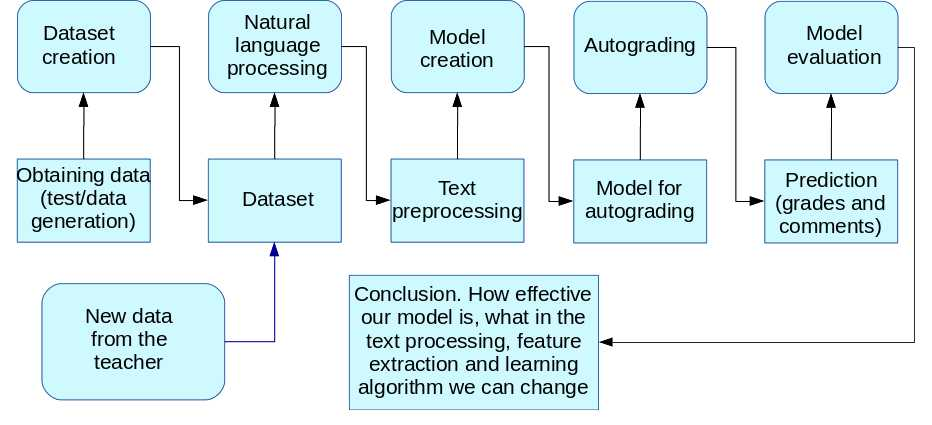
\includegraphics[width=1.0\textwidth]{img/workflowEN}
    \caption{A general workflow for an ASAG system developement ~\cite{Burrows}.\label{fig:workflowEN}}
\end{figure}

\begin{preview}
\centering
\tikzset{every picture/.style={xscale=0.7,transform shape}}
  \begin{gantt}{6}{10}
    \begin{ganttitle}
    \titleelement{1995-2000}{2}
    \titleelement{2000-2005}{2}
    \titleelement{2005-2010}{2}
    \titleelement{2010-2015}{2}
    \titleelement{2015-2018}{2}  
    \end{ganttitle}
    \ganttbar{\textbf{Concept mapping}}{0}{7.5}
    \ganttbar{\textbf{Information extraction}}{2.5}{4}
    \ganttbar{\textbf{Corpus-based methods}}{2.9}{3.2}
    \ganttbar{\textbf{Machine learning}}{5.4}{4.6}
    \ganttbar{Deep learning}{9}{1}
  \end{gantt}
\end{preview}

\subsubsection{Concept/facet mapping}

The oldest direction in ASAG research is, in its pure form, mostly interesting from the historical point of view, for it is not being actively used nowadays. The main idea is searching for the presence/absence of certain concepts those students can mention on their answers. This can be used either on a sentence or facet level. The facet normally contains three or two words ~\cite{Burrows}. This approach is in a way similar to textual entailment, because entailment also concerns, if one sentence means the same that another, contains the same concept -- entails it -- or not.\\

The biggest disadvantage of this approach for ASAG is that it can detect the presence of the concept, but not if it was mentioned in a correct way ~\cite{Dzikovska}. For example, a student can write "Q: What is PCA? A: PCA is a method that affects dimensionality. It increases it.", which is incorrect, but the algorithm may still accept or partially accept this answer, because PCA really affects the dimensionality and it might match the concept, whereas the second part can be not accounted into the same concept estimation.\\

The first concept mapping system was developed by \textbf{Burstein} in 1996 ~\cite{Burrows}. It uses  Lexical Conceptual Structure representation, which means that the system detects a presence of certain words and grammatical structures. The approach was rather limited, because it only allowed a certain type of question -- the  hypothesis-style, which means that the answer to this question must contain several explanations of the hypothesis.\\

Another mapping system is Automatic Text Marker (\textbf{ATM}). It operates with facets: ATM divides example and students' answers into pieces containing a couple of words each, and estimates the number of common concepts in those small parts of example ans students' answers. It is important that a higher weight can be assigned to the piece with a keyword ~\cite{Burrows}.\\

A concept mapping system developed by ETS is called a Concept Rater or \textbf{c-rater}. It focuses on sentence-level comparison of example and students' answers. An example answer is intentionally formulated in such a way that each sentence contains only one concept. Sentence comparison is rule-based and includes a paraphrase recognizer that can distinguish syntactic variations, pronoun references, morphological variations, and synonyms. Moreover, it uses spelling correction ~\cite{c-rater}. \\

Later concept mapping stated including machine learning. \textbf{Wang} in ~\cite{Wang} compares pure heuristics-based concept mapping with  data-driven classification by support vector machines (SVM) and combination of those two methods. In a combination of methods SVM was used with bag-of-words features, whereas pure machine learning used unigrams and bigrams. The best result was reached using the combination of methods.\\

Table \ref{CFM} shows the comparison of methods above. Accuracy between certain numbers means that the algorithm gives different correlation with human graders on different datasets.

\begin{table}[h!]
\centering
\caption{Concept/facet mapping systems}
\label{CFM}
\begin{tabular}{|l|l|l|l|}
\hline
 System & Year & Approach & Accuracy \\ \hline
 Burstein & 1996 & lexical conceptual structure representation & 48\% to 83\% \\ \hline
 ATM & 2001 & weighted comparison of few-words facets & unknown \\ \hline
 c-rater & 2003 & sentence-level paraphrase recognition & 87\% to 94\% \\ \hline
 Wang & 2008 & concept mapping with SVMs & 92\% \\ \hline
\end{tabular}
\end{table}

\subsubsection{Information extraction}

Information extraction (IE) has already been cosidered in NLP section of thei work. For ASAG it is also basically a pattern or fact template matching, template merging and resolution of referential ambiguities ~\cite{Burrows}, ~\cite{Pulman}. It allows to extract a structures information from unstructured sources. A significant advantage of this approach is its robustness. To certain extend it is immune to grammatically wrong sentences and therefore requires less text preprocessing. The main IE approches are listed below ~\cite{Hasanah}, ~\cite{Pulman}: 

\begin{itemize}
\item \textbf{parse tree matching} uses specific templates for correct and wrong answers. Each answer is being preprocessed and compared to templates with different grades. An example of such approach is \textbf{AutoMark} grader.
\item \textbf{regular expression matching} applies a regular expression patter to all elements of the students' answers. Examples of such approach are \textbf{WebLAS} and \textbf{PMatch} graders:
\begin{itemize}
\item  WebLAS is an older system. It automatically extracts the patterns from example answers and then offers the grader to approve it and its synonyms and give a certain weight to each patter. Then the algorithm goes through the students' replies and matches the patterns. Thereby it is possible to give a wide range of grades -- based on how much patterns were matched and their weight \cite{Burrows}. 
\item PMatch is suitable only for very short answers -- not longer than one sentence. The system can match short and simple word sequences. It can inform students that words in their replys are either misspelled or unknown to the system and offer spelling correction options ~\cite{Hasanah}, ~\cite{Burrows}.
\end{itemize}
\item the main idea of \textbf{boolean phrase matching} is matching of key-phrases between an example and answers to grade. To be able to deal with synonyms and word forms the systems with boolean matching use thesaurus and lemmatization. Phrases with the same meaning are added to the needed sentence representation as "or" and the required ones -- as "and" ~\cite{Hasanah}. An example of this is shown in Fig.\ref{fig:AndOr}. It is taken from the work by \textbf{Thomas} ~\cite{Thomas}, which describes an example of such an autograding system. Due to "or" the system has a certain flexibility, however, as a correct answer it could only accept a perfect match with one of the phrases from the tree.
\begin{figure}[h!]
  \centering
  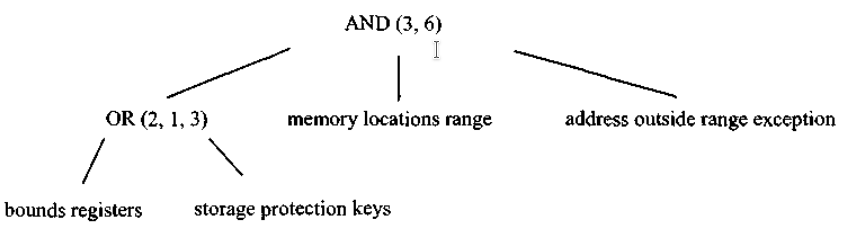
\includegraphics[width=0.8\textwidth]{img/AndOr}
    \caption{ An example of boolean and/or tree for the answer that must contain the following: "bounds registers", "range memory locations,", "address outside range exception" ~\cite{Thomas} }\label{fig:AndOr}
\end{figure}
\item \textbf{syntactic pattern matching} is a variety of methods using different syntactic structures:
\begin{itemize}
\item \textbf{auto-marking} requires specifically developed grammars those contain the hand-crafted patterns to match. This system is hard to use for people unfamiliar with the rules those were used for grammar construction ~\cite{Hasanah}.
\item In \textbf{Oxford-UCLES} system Pulman and Sukkarieh uses Hidden Markov part-of-speech model in combination with Noun Phrase and Verb Group finite state machine. Their approach excludes templates merging and ambiguity resolution, because they assume that the student replies in their dataset don't contain unnecessary information and ambiguous phrases. IE is combined with such machine learning methods as Naive Bayesian learning, inductive logic programming and decision trees. The best result was achieved with Naive Bayesian learning ~\cite{Pulman}.
\item \textbf{IndusMarker} as well as auto-marking uses specifically constructed grammars for word- and phrase-level matching, but also includes spell checking and correction. The system developers introduced a "Question Answer Markup Language" where the users can input the correct answers ~\cite{Burrows}.
\end{itemize}
\item \textbf{syntactic-semantic pattern matching}:
\begin{itemize}
\item \textbf{eMax} uses both syntactic and semantic analysis. User of the system must provide one or multiple correct answers and highlight important elements of them. It is important that the system provides a confidence level, so a human grader could check the low-confidence answers him/herself ~\cite{Burrows}, ~\cite{Hasanah}.
\item \textbf{FreeText Author} operates on a sentence-level. Every sentence is being semantically analyzed and the system returns a certain feedback that is compared to the feedback from the syntactic-semantic templates those are automatically created based on example answers. User of the system can specify keywords and accepted synonyms. The system has a user-friendly interface and it is easy to use ~\cite{Burrows}, ~\cite{Hasanah}.
\end{itemize}
\item \textbf{semantic word matching} is based on individual terms matching. An example of such a system is \textbf{Auto-Assessor}. To rate answers it uses such NLP tools as bag-of-words, WordNet.NET and SharpNLP. The system can only accept one example answer, but of this example it automatically generates a range of acceptable solutions. It grades based on can only grade one-sentence answers. Auto-Assessor has a user-friendly interface ~\cite{Burrows}, ~\cite{Hasanah}. 
\item \textbf{Lexical Resource Semantics (LRS) representation matching} system -- \textbf{CoSeC-DE} -- was developed by Hahn in 2012. The system uses Corpus of Reading Comprehension Exercises in German (CREG) ~\cite{CREG}. The answers are preprocessed using TreeTagger and dependency parser MaltParser and afterwards the system creates syntax-semantics-interface representations and then builds lexical resource semantics representations. Comparison of example and the answer to grade is performed by alignment afterwards. It is more accurate than bag-of-words model, because it allows to avoid consider a sentence of a higher level and avoid such problems: consider the sentences below: "CoSeC-DE is more advanced than AutoMark", "CoSeC-DE outperforms AutoMark", "AutoMark is more advanced than CoSeC-DE". Bag-of -words would assume that the first and third sentences are the same and the second one is different, whereas the first two are the same and the third one contradicts them. CoSeC-DE evaluates these sentences correctly  ~\cite{Hahn}.
\end{itemize}


\begin{table}[h!]
\centering
\caption{Information extraction systems}
\label{IE}
\begin{tabular}{|l|l|l|l|}
\hline
 System & Year & Approach & Accuracy \\ \hline
 AutoMark & 2002  & parse tree matching & 92.5\% \\ \hline
 WebLAS & 2002  & regular expression matching  & unknown \\ \hline
 PMatch & 2012  & regular expression matching & 90\%  \\ \hline
 Thomas & 2003  & boolean phrase matching & 86\% \\ \hline
 auto-marking & 2003  & syntactic pattern matching &  88\% \\ \hline
 Oxford-UCLES & 2005  & syntactic pattern matching &  87\% \\ \hline
 IndusMarker & 2008  & syntactic pattern matching & 96\% \\ \hline
 eMax & 2009  & syntactic-semantic pattern matching &  unknown \\ \hline
 FreeText Author & 2009  & syntactic-semantic pattern matching &  unknown \\ \hline
 Auto-Assessor & 2011  & semantic word matching  &  unknown \\ \hline
 CoSeC-DE & 2012 & LRS representation matching &  86.3\% \\ \hline
\end{tabular}
\end{table}

From the Gantt chart above and Burrows's review paper one can see that this research direction tends to stay in the past as well as the concept mapping, but Hasanah ~\cite{Hasanah} in 2016 year's paper argues that it is a valid method that can be used in combination with corpus-based methods, which can help to deal with synonyms, in the future.

\subsubsection{Corpus-based methods}

This group of methods is widely used for analyzing of large texts and it has already been considered in AES section, but can also be useful for ASAG, because it allows a better paraphrasing detection by efficient interpreting of synonyms ~\cite{Burrows}. These are statistical methods those use information from the large amount of text, so short answers should be preprocessed in order for corpus-based methods to be applied. Below the most significant corpus-based methods are considered.\\

\textbf{Atenea} system uses a weighted combination of an extended version of BiLingual Evaluation Understudy (BLEU) metric and LSA ~\cite{ERB}. LSA has already been considered in AES section. BLEU in turn was initially used in machine translation, but later it become used in all fields of machine text-processing including ASAG systems. The key concept of this metric is a modified unified n-gram precision (MUP) measure: all n-grams (consequtive sequences of n words in the sentence) and number of their occurances are taken into account, n-grams of certain type are summed up and divided by the total number of n-grams. It is calculated in the following way ~\cite{BLEU}:\\

\begin{equation} \label{eq:MUP}
MUP_n = \frac{\sum\limits_{C \in \{AnswerSentences\}} \sum\limits_{n-gram \in C} count_{matches}(n-gram)}{\sum\limits_{C' \in \{AnswerSentences\}} \sum\limits_{n-gram \in C'} count_{matches}(n-gram')}.
\end{equation}

\begin{equation} \label{eq:BP}
BP = \begin{cases}
   1 &\text{if $c>r$}\\
   e^{1-r/c} &\text{if $c \leq r$}
 \end{cases},
\end{equation}

where BP is a brevity penalty, c -- length of the student's answer and r -- effective reference corpus length.

\begin{equation} \label{eq:BLUE}
SIM_{BLUE} = BP \times e^{\sum^N_{n=1}w_n \times log(MUP_n)},
\end{equation}

where N is a maximum size of an n-gram and $w_n$ -- weight of the corresponding n-gram size. For estimation of BLUE similarity usually $log(SIM_{BLUE})$ is used. \\

For convenience of the reader, these and further similarity measures are summarized in a table \ref{sim} in the "State of the art summary" section.\\

An extended version of BLEU -- Evaluating Responses with BLEU (ERB) adds recall accommodating to precision that uses modified brevity penalty (MBP) factor. The ERB similarity is calculated in the following way ~\cite{ERB}:

\begin{equation} \label{eq:ERB}
SIM_{ERB}(answer) = MBP(answer)\times e^{\sum^{N}_{n=0}\frac{log(MUP(n))}{N}},
\end{equation}

where n -- number of n-grams, N -- highest possible value of n. \\

Another system for corpus-based ASAG is \textbf{Willow} developed on the base of Atenea ~\cite{Willow}. The system is different from the previous ones, because it extensively uses various shallow NLP techniques, such as stemming and lemmatization, disambiguation, and multiword term identification. Basically, Willow is based on ERB with an NLP preprocessing. The architecture of the system is shown in Fig. \ref{fig:WillowArch}. It doesn't include LSA part explicitly, but it is normally being used in combination with LSA: LSA + Willow (NLP (stemming + removal of closed-class words + no disambiguation) + ERB). The combination is calculated in the following way:

\begin{equation} \label{eq:Willow}
SIM_{Willow} = \alpha \times SIM_{PureWillow} + (1 - \alpha \times SIM_{LSA}),
\end{equation}

where $\alpha$ is a parameter that defines the weights of LSA and Willow parts, the best result was reached with $\alpha = 0.489$. WordNet and British National Corpus (BNC) for English and EuroWordNet for Spanish were used for LSA.\\

 \begin{figure}[h!]
  \centering
  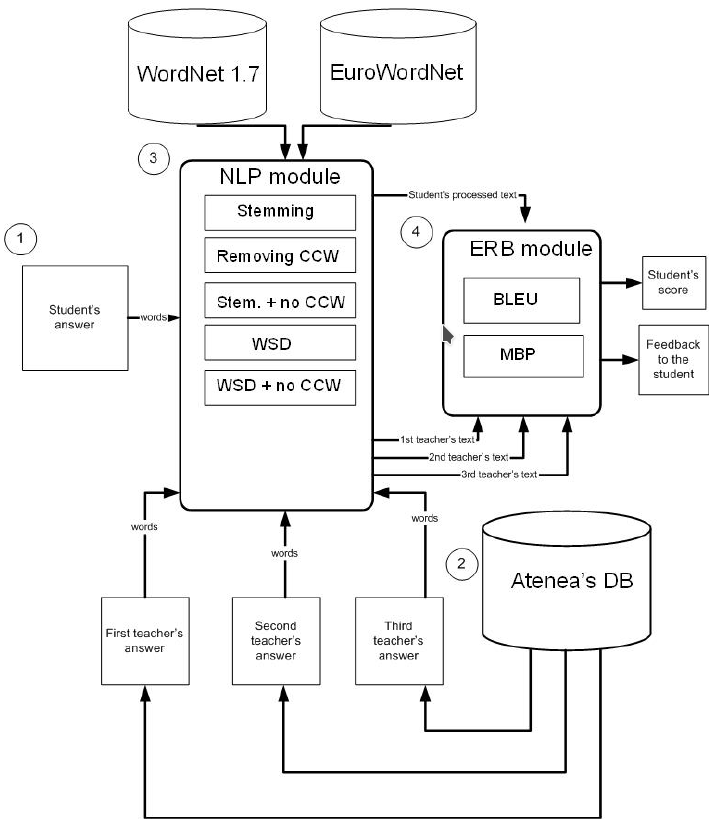
\includegraphics[width=\textwidth]{img/WillowArch}
    \caption{ Willow's architecture ~\cite{Willow}, where "CCW" is "closed-class words" and "WSD" -- word sense disambiguation.}\label{fig:WillowArch}
\end{figure}

The system had a user-friendly interface (see Fig. \ref{fig:Willow}) and it worked with English and Spanish.\\

\begin{figure}[h!]
  \centering
  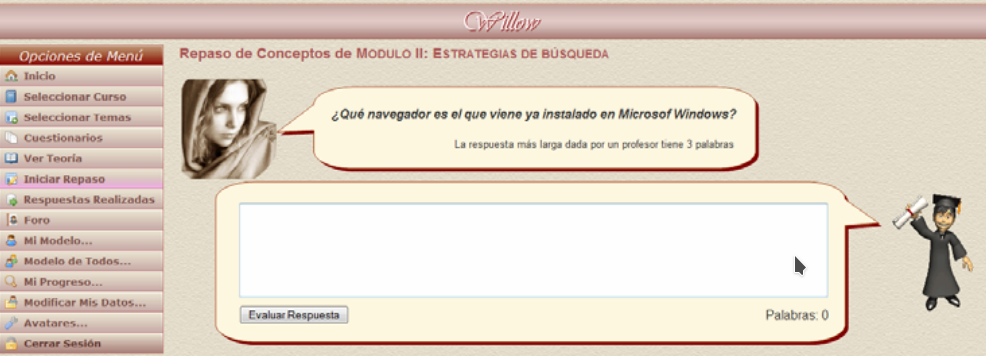
\includegraphics[width=\textwidth]{img/Willow}
    \caption{ Interface of Willow ~\cite{Willow}. }\label{fig:Willow}
\end{figure}


In \textbf{Short Answer Measurement of Text (SAMText)} author uses modified LSA. He finds the regular LSA unsuitable for ASAG due to the following reasons ~\cite{SAMText}:
\begin{itemize}
\item LSA is ineffective when the answer is shorter than around 200 words, which is often the case in ASAG.
\item Relevant corpus doesn't always exist. LSA trained on general texts can be rather useless for specific areas and it is not always easy to find a large enough corpus for this specific area.
\item Most of the existing LSA-based systems require large pregraded datasets. Therefore, a solution might only work well on some specific dataset and an attempt to extend it to a new area of knowledge would fail. That is one of the reasons why it doesn't make much sense to compare the accuracy of various ASAG systems given in the published papers -- everybody uses their own dataset, which can be overly convenient for their method, and often there is no published code to test the solutions on the similar datasets. 
\item To use LSA one must find an optimal dimensionality.
\end{itemize}
Whereas a regular LSA uses a large corpus to model semantic relatedness, the given LSA modification is based on inverted index data structure, which requires general-corpus and topic-specific keywords to create the corpora. The advantage of the approach is that it allows to use a subject-specific sublanguage  instead of the whole language. Thereby, modified LSA can work properly with short answers and only requires a few example answers ~\cite{Burrows}.\\

\textbf{Mohler} ~\cite{Mohler} focuses on unsupervised ASAG systems and evaluates ten of them on the same dataset obtained from  Data Structures course. It is important, because, as it was mentioned above, it is usually hard to compare the  systems tested on completely different datasets. Moreover, the dataset was published and thereby the other authors later also have the opportunity to use this dataset to evaluate their algorithms ~\cite{Sultan}, which allows to obtain comparable results. The following methods were evaluated: 
\begin{itemize}
\item knowledge-based methods with the following maximum similarity metric:
\begin{equation} \label{eq:maxsim}
maxsim(W,C) = max SIM_x(W,w_i),
\end{equation}
where $C$ is a word class, W -- a word of the class from the example answer, $w_i$ -- a word of the class from the student answer, $SIM_x$ -- one of the following similarity measures:
\begin{itemize}
\item shortest path:
\begin{equation} \label{eq:shortestPath}
SIM_{shortestPath} = \frac{1}{length},
\end{equation}
where $length$ is the shortest path between the concepts calculated based on node-counting. Accuracy: 44.14\%.
\item C-Rater (has already been considered in "Concept/facet mapping" section):
\begin{equation} \label{eq:c-rater}
SIM_{c-rater} = -log \frac{length}{2 \times D},
\end{equation}
where $length$ is calculated similar to the shortest path approach and D is the maximum depth of the taxonomy. Accuracy: 22.31\%.
\item Lesk:
\begin{equation} \label{eq:Lesk}
SIM_{Lesk} = f(two\_concepts\_overlap).
\end{equation}
Accuracy: 36.3\%.
\item Wu and Palmer:
\begin{equation} \label{eq:Wu}
SIM_{Wu} = \frac{2 \times depth(least\_common\_subsumer)}{depth(concept_1) + depth(concept_2)},
\end{equation}
where the concepts are from WordNet taxonomy. Accuracy: 33.66\%.
\item Resnik:
\begin{equation} \label{eq:Resnik}
SIM_{Resnik} = -log P(least\_common\_subsumer),
\end{equation}
where $P(concept)$ is a probability to find an instance of the concept in a given corpus. Accuracy: 25.20\%.
\item Lin:
\begin{equation} \label{eq:Lin}
SIM_{Lin} = \frac{2 \times log P(least\_common\_subsumer))}{log P(concept_1) + log P(concept_2)}.
\end{equation}
Accuracy: 39.16\%.
\item Jiang and Conrath:
\begin{equation} \label{eq:Jiang}
SIM_{Jiang} = - \frac{1}{log P(concept_1) + log P(concept_2) - 2 \times log P(least\_common\_subsumer) }.
\end{equation}
Accuracy: 44.99\%.
\item Hirst and St-Onge:
\begin{equation} \label{eq:Hirst}
SIM_{Hirst} = f(strength\_of\_pair\_of\_synonym\_sets),
\end{equation}
which is based on lexical chains detection in WordNet taxonomy. Accuracy: 19.61\%.
\end{itemize}
The implementation of the methods above is WordNet-based.
\item corpus-based methods :
\begin{itemize}
\item LSA (considered in details in "AES" section) trained on BNC and English Wikipedia (September 2017 version). For implementation of LSA InfoMap package (\url{http://infomap-nlp.sourceforge.net/}) is used. Accuracy: 67.35\% -- on reduced computer science Wikipedia corpus with adding new good students' answers to the examples list.
\item Explicit Semantic Analysis (ESA or ESA Wikipedia) -- concept-vector features approach trained on Wikipedia (September 2017 version) corpus, each article is a concept vector. This algorithm is implemented by the authors themselves based on work by Gabrilovich and Markovitch ~\cite{Gabrilovich}. Accuracy: 64.98\% -- on full Wikipedia corpus with adding new good students' answers to the examples list.
\end{itemize}
It was shown that the accuracy of LSA strongly depends on the size of training corpus and on how close the corpus topic is to the topic of exam, i.e. the better results for the Data Structures test was obtained using domain-specific corpus that contained Wikipedia articles on computer science. However, for ESA the size is more important and it performs worse on a smaller domain-specific corpus. Also, in addition to the example correct answers the system added the best student answers to the list of examples, which helped to improve the quality of grading significantly. 
\end{itemize}

It is interesting that the result of LSA, which was said to be unsuitable for ASAG in Bukai's work ~\cite{SAMText} shows the best results in Mohler's work ~\cite{Mohler}. However, the best result is 67.35\%, therefore it is still questionable, if LSA сan be used for ASAG. \\

As it was shown by Mohler ~\cite{Mohler}, LSA performs better when trained on domain-specific corpus. Therefore, \textbf{Klein} ~\cite{Klein} trains LSA on even more specific corpus that consists only of partially manually-graded student's answers. To determine the distance between the answers, a linear combination of cosin and Euclidean similarities was chosen:

\begin{equation} \label{eq:cos}
SIM_{cos} = \frac{\pmb{answer_1} \times \pmb{answer_2}}{||\pmb{answer_1}|| \times ||\pmb{answer_2}||},
\end{equation}
\begin{equation} \label{eq:Euclidean}
SIM_{Euclidean} = 1 - \sqrt{\sum^k_{i=1}(answer_{1_i} - answer_{2_i})^2},
\end{equation}
\begin{equation} \label{eq:combinedCE}
\begin{array}{l}
SIM_{combined} = \alpha  \times SIM_{Euclidean}(\pmb{answer_1}, \pmb{answer_2}) + \\ + (1-\alpha) \times SIM_{cos}(\pmb{answer_1}, \pmb{answer_2}),
\end{array}
\end{equation}\\
 where $\alpha$ is a parameter between 0 and 1 that allows to assign a weight to the distances. However, it was shown that the best result is reached when $\alpha = 1$, i.e. when only cosine similarity is used. \\
  
The system would find the graded answer, which is the most similar to the student's answer, and gives it the corresponding grade. It is important that in case if there is no graded assignment that is similar enough, the student's answer is marked as "unassigned". LSA here is used in combination with clustering. Three clustering methods to choose the assignments to grade manually were used:
\begin{itemize}
\item random choice of assignments to be graded manually
\item k-means clustering to divide the students' answers into semantically-similar clusters: one or two answers from each cluster should be graded manually
\item modified similarity-based Min-Max algorithm: first answer to grade manually is chosen randomly and the new ones are chosen in such a way that the answer should be the least similar to the closest answer in already built manually-graded set:\\ $index = argmin_{index}(max_j (SIM_{combined} (\pmb{answerToAdd_{index}}, \pmb{gradedAnswer_j})))$
\end{itemize}
The Min-Max algorithm was shown to be the most efficient and k-means was on the second place: the total amount of answers was 49, Min-Max algorithm allowed to reduce the number of manually graded answers to 35, k-means -- to 40 and random choice -- between 41 and 45. The accuracy of the grading is fairly high -- between 80\% and 95\%. However, to really reduce the teacher's workload, it would require a lot of pregraded works from previous exams those must be similar to the current one, otherwise it only allows to reduce the number of works to grade by around 20\%-30\%, which doesn't worth the effort. \\

The work of \textbf{Noorbehbahani} ~\cite{Noorbehbahani} deserves a special attention, for it contains a good description of various metrics:

\begin{itemize}
\item n-gram co-occurrence --  number of similar n-grams:\\
$SIM_{n-gram} = \frac{N_{sim}}{N_{total}},$\\
where $N_{sim}$ -- number of matching n-grams between the student's and example answers and $N_{total}$ -- total number of n-grams in student's answer.
\item BLUE -- has already been considered above in this section -- in the description of Atenea system, see equation \ref{eq:BLUE}. In addition to that
Noorbehbahani mentions the following drawbacks of the system ~\cite{Noorbehbahani}:
\begin{itemize}
\item BLUE only recognizes exactly-matching words, which means that it discards even misspelled words, and will certainly ignore synonyms;
\item all words have the same weights, which means that the essential for the meaning of the answer special terms would have as much meaning as articles or transition words;
\item the system compares the student answer with all reference answers and counts matches from different references;
\item brevity penalty punishes all answers those are longer than the reference ones, which doesn't always makes sense.
\end{itemize}
\item M-BLUE -- the system proposed by Noorbehbahani. It is based on the same idea, but includes the following modifications:
\begin{itemize}
\item spelling correction;
\item acceptance of synonym-n-grams, understanding of paraphrasing: the system generates synonym example answers based on the given reference answers in such a way that it is as close as it is possible to the student answers, but still keeps the meaning of the reference answers;
\item weighting of the n-grams by their importance, i.e. special terms should have higher weights, whereas an n-gram like "and the" can have a nearly-zero weight;
\item the system compares student's answers with all the example answers, but the final similarity measure is calculated only with the most similar one.
\item brevity penalty is calculated based on weights, because the length of the answer doesn't help to estimate the correctness;
\item the final M-BLUE similarity measure is calculated in the following way:
\begin{equation} \label{eq:M-BLUE}
SIM_{M-BLUE} = \lambda \times BP_r \times SIM_{M-BLUE} + (1 - \lambda) \times S_0,
\end{equation}
where $BP_r$ is a modified weighted brevity penalty, $SIM_{BLUE_ra}$ -- weighted similarity measure between a student answer and one reference answer, $S_0$ --  measure for calculating the common-words order similarity and $\lambda$ is a similarity components weight parameter, which is taken in range between 0.5 and 1. In Noorbehbahani's work $\lambda = 0.85$ was chosen experimentally. The whole derivation of the equation \ref{eq:M-BLUE} is intentionally omitted, because the meaning of the equation members is clear from the list items above and the formulas for them can be found in ~\cite{Noorbehbahani}.
\end{itemize}
\item ERB -- has already been considered above in this section -- in the description of Atenea system, see equation \ref{eq:ERB}.
\item Recall-oriented understudy for gisting evaluation (ROUGE) was initially developed for evaluation of quality of the summaries. There are the following implementation of ROUGE:
\begin{itemize}
\item ROUGE-N -- estimates n-gram with $n>1$ co-occurrences, similar to BLEU.
\item ROUGE-L -- finds and calculates the length of longest common subsequence of two answers.
\item ROUGE-W -- finds similar subsequences and takes them into account according to weights.
\item ROUGE-S -- uses skip-bigram. Skip-grams is a method in which "n-grams are still stored to model language, but they allow for tokens to be skipped" ~\cite{Skip-gram}. Guthrie  ~\cite{Skip-gram} defines k-skip-n-grams for a sentence containing words $w_1,w_2,...,w_n$ in the following way:\\
$\{w_{i1},w_{i2},...,w_{in} | \sum_{j-1}^n i_j - i_{j-1} < k\}$.\\
is strictly higher than one. For better understanding of the concept the following example can be made. For a sentence "A new art colour for our Irish
poets: snotgreen. " ~\cite{Ulysses} it would be so: bi-grams = {"A new", "new art", "colour for", "for our", "our Irish", "Irish
poets", "poets snotgreen"} and 2-skip-bi-grams = {"A new", "A art", "A colour", "new art", "new colour", "new for", "for our", "for Irish", "for poets", "our Irish", "our poets", "our snotgreen", "Irish poets", "Irish snotgreen",  "poets snotgreen"}. One can see that in many cases it creates senseless sequences of the words like "A art", however, k-skip-n-gram "for Irish" would make total sense, because the sentence without word "our" is as valid as the initial one. Moreover, the wrong k-skip-n-grams are too random and often grammatically senseless, that is why they can with very low probability create false positives, which shows that it is at least harmless to use them.
\item ROUGE-SU -- uses the same idea that ROUGE-S, but also takes into account unigrams.
\end{itemize}
\item Combination of LSA and n-grams -- answers are broken into sentences, each of them is a vector for LSA and closeness of the answers is evaluated as a cosin distance. Separately n-gram n-gram co-occurrence is calculated. After this, two similarities are combined:\\
\begin{equation} \label{eq:LSA+n-grams}
SIM_{LSA+n-grams} = \frac{SIM_{LSA} + SIM_{n-gram}}{2}.
\end{equation}
The method can be modified by a more complex -- weighted -- calculating of the similarity.
\end{itemize}

The dataset used in this paper was obtained from a computer science e-learning course. It contained 45 questions, 300 example answers and 237 student's answers.\\

There were several important papers on corpus-based methods published 2012. The first one by \textbf{Li} ~\cite{Li} concentrates on various similarity metrics, which allows us to extend the list of the metrics given by Mohler and Noorbehbahani. The following similarity metrics are considered:

\begin{itemize}
\item cosine similarity -- has already been considered above in this section -- in the description of Mohler's system. \\
Accuracy: 75.3\%.
\item Jaccard similarity -- percent of intersection of two sets (words of answers):
\begin{equation} \label{eq:Jaccard}
SIM_{Jaccard} = \frac{answer_1 \cap answer_2}{answer_1 \cup answer_2}.
\end{equation}
Accuracy: 73.9\%.
\item S{\o}rensen-Dice coefficient -- a number of overlap words in two answers:
\begin{equation} \label{eq:Dice}
SIM_{Dice} = \frac{2 \times (answer_1 \cap answer_2)}{|answer_1| + |answer_2|}.
\end{equation}
Accuracy: 76.6\%.
\item Manhattan similarity -- introduced by Li for ASAG. Each answer is represented by a vector, e.g. $ \pmb{answer_1} = (answer_{1_1}, answer_{1_2},..., answer_{1_n})$, where n is a length of the answer in words. The similarity is calculated between the student's answer and multiple example answers in the following way:
\begin{equation} \label{eq:Manhattan}
SIM_{Manhattan} = 1 - \sum^n_{k=1}|answer_{1_k} - answer_{2_k}| / m,
\end{equation}
where m is the total number of words in two answers.\\
As a reference answer the most similar example answer is chosen, i.e. similarity between this and student answer would be taken into account for grading.\\
Accuracy: 76.2\%.
\item Keywords coverage rate -- basically it is a count of present and absent keywords or their synonyms. For this Levenshtein distance ("minimum number of operations needed to transform one string into the other" ~\cite{Gomaa}) is used, because it allows to evaluate substitutions and deletions in strings. \\

\begin{equation} \label{eq:Levenshtein}
SIM_{Levenshtein} = \frac{max(length(currentWord,keyword)) - minLev}{length(keyword)},
\end{equation}
where $minLev$ is the distance between the current keyword the most similar word in a student's answer. If it is larger or equal to the minimal length of the two words, $SIM_{Levenshtein}$ nullifies. 
\begin{equation} \label{eq:keywordCover}
keywordCoverage = \sum_{i} SIM_{Levenshtein} / numberOfKeywords,
\end{equation}
Accuracy: 64.6\%.
\end{itemize}

The similarity measures were tested separately and then combined with different weights those were determined by linear regression.\\

A distinctive feature of this paper is that they evaluate non written, but spoken answers, which makes preprocessing harder, and requires speech-recognition tools instead of, for example, spelling correction. However, the rest of the work is similar to the regular written ASAG. The author claims that the accuracy of the method is 77.8\% and it is very impressive, eepesially taking into account that the correlation between the human raters was 80.5\%. However, the used dataset was rather simple. Here are some examples of the answers: "Hello, Xiao Li! This is Bill speaking. What's up?", "Good idea! How much is a ticket?", "All rightˊSee you then! Bye!" ~\cite{Li}. It would be a valid assumption that the results on more complex dataset, e.g. Mohler's one, would be much lower, because even the keyword spotting alone has given 64.6\% correlation with a human grader. Though the results of this work might be not very impressive, it is a good article to move from corpus-based methods to machine learning, because the approach of using various distances as different features will be helpful for machine learning.\\

Another paper published in 2012 by \textbf{Gomaa} ~\cite{Gomaa} also uses a combination of several types of methods -- on string-based and corpus-based. String-based methods are represented by the following:
\begin{itemize}
\item Character-based distance measures
\begin{itemize}
\item Levenshtein distance -- described in the work considered before.
\item Jaro-Winkler distance -- calculates the number of similar characters in two answers taking into account their order. Similarity is calculated in the following way ~\cite{Jaro}
\begin{equation} \label{eq:Jaro}
SIM_{Jaro} = \begin{cases}
   0 &\text{0 if $m = 0$}\\
   \text{$\frac{1}{3}(\frac{m}{answer_1} + \frac{m}{answer_2} + \frac{m - t}{m})$}&\text{otherwise},
 \end{cases}
\end{equation}
where m is the number of matching characters and t -- half of the total transpositions number.
\item Needleman-Wunsch algorithm -- dynamical-programming algorythm initially used for protein or nucleotide sequences similarity calculations. It searches for the best alignment over the whole two answers.
\item Smith-Waterman algorithm -- also from dynamic programming, looks for similarities over conserved domain of two answers. 
\item n-gram co-occurrence -- considered above in the description of Noorbehbahani's work.
\end{itemize}
\item Term-based distance measures
\begin{itemize}
\item Manhattan distance -- considered above in the description of Li's work.
\item cosine similarity -- considered above in the description of Mohler's system.
\item S{\o}rensen-Dice distance -- considered above in the description of Li's work.
\item Euclidean distance -- considered above in the description of Mohler's system.
\item Jaccard similarity -- considered above in the description of Mohler's system.
\item Matching Coefficient -- number of non-zero values over the term axes those are similar for two answer-vectors.
\item Overlap coefficient -- modified S{\o}rensen-Dice distance: if only a subset of one answer is similar to the whole other answer, these answers are 100\% match.
\end{itemize}
\end{itemize}

Corpus-based similarity methods are represented by the following:

\begin{itemize}
\item LSA -- considered above in AES section.
\item ESA -- considered above in the description of Mohler's system.
\item Pointwise Mutual Information - Information Retrieval ( ) -- uses  AltaVista's Advanced Search query syntax to calculate the matching between word pairs by calculating the probability of co-occurrence of the words based on web pages corpus.
\item extracting DIstributionally related words using CO-occurrences (DISCO) -- Java application for calculating similarity between words or short texts, finding the most similar words in texts, e.g. "smart" and "clever", and finding the related words, e.g. "beer" $\rightarrow$ "K\"olsch", alcohol, foam, barrel. It requires a database of word similarities (word space) precalculated on a large text corpora by "DISCO Builder". It is similar to word2vec --  log-bilinear prediction-based bag-of-words and skip-n-gram algorithms for vectorizing words developed by Google  ~\cite{word2vec} -- and Global Vectors for Word Representation (GloVe) -- log-bilinear regression unsupervised algorithm for word vectorization ~\cite{GloVe}. Architecture of the system is shown in Fig. \ref{DISCO}. DISCO Builder is trained on Wikipedia and BNC. 
\begin{figure}[h!]
  \centering
  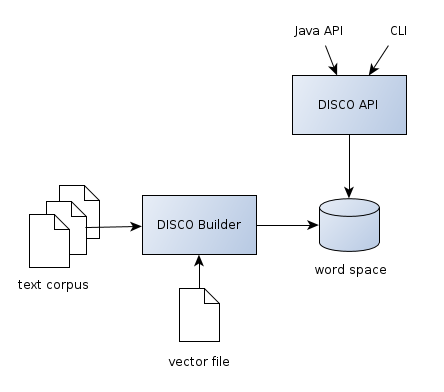
\includegraphics[width=0.8\textwidth]{img/DISCO}
    \caption{ Architecture of DISCO ~\cite{DISCO}. }\label{fig:DISCO}
\end{figure}
\end{itemize}

ASAG is performed in three stages:
\begin{itemize}
\item answer similarities are calculated by all string-based methods above.
\item DISCO similarities are calculated, at the same step lammatization and stop-words removal are made.
\item combination of first two steps and deriving the grade based on maximum and average overall similarities
\end{itemize}
To evaluate the efficiency of the introduced methods, Mohle'r dataset is used. The best human-computer correlation among string-based methods was achieved by n-gram co-occurrence -- 39.8\%. The best DISCO result was shown after training on Wikipedia corpus -- 47.5\%. The three methods mentioned above were combined and the total result reached 50.4\%. This work shows not very high results in comparison to many other papers, however, there are several important points:
\begin{itemize}
\item it uses Mohler's dataset, which  makes the result comparable. Moreover, the obtained result is not that low if we compare it to the other algorithms trained on the same data.
\item The algorithm was trained on whole Wikipedia corpus. It is very likely that the result would be better if only computer science Wikipedia would have been used, as it helped to improve LSA's performance in Mohler's work.
\item The work also shows the importance of combination of various metrics and methods and thereby leads to using them as features in machine learning.
\end{itemize}
 
Table \ref{Corpus} shows the comparison of various corpus-based methods those are in part of the cases combined with various similarity metrics. A dataset column was not added intentionally, because most of the works use their own datasets. The works using Mohler's dataset marked as "(MD)".
 
\begin{table}[h!]
\centering
\caption{Corpus-based systems and metrics}
\label{Corpus}
\begin{tabular}{|l|l|l|l|}
\hline
 System & Year & Approach & Accuracy \\ \hline
 Atenea & 2004 & ERB + LSA & 50\% \\ \hline
 Willow & 2006 & ERB + LSA + NLP & 56\% \\ \hline
 SAMText & 2006 & modified LSA & 69\%-72\% \\ \hline
 Mohler & 2009 & LSA & 67.35\% (MD) \\ \hline
 Klein & 2011 & LSA + clustering &  80\%-95\% \\ \hline
 Noorbehbahani & 2011 & M-BLEU & 85\% \\ \hline
 Gomaa & 2012 & bag of words & 50.4\% (MD) \\ \hline
 Li & 2012 & Approach & 77.8\% \\ \hline
\end{tabular}
\end{table}
 
\subsubsection{Machine learning}

Machine learning (ML) requires a preprocessing that would allow to retrieve features for further reduction of the ASAG task to regression or classification problem. Previous section of the work focused on corpus-based methods and similarity metrics. First works were mostly using one or two metrics combined with certain weights. However, the latest works started using a combination of several techniques with automatically chosen wights and it was shown that this approach gives better results. This led to an important idea of combination of several techniques as features for further machine learning. And moreover, to an idea of combination of several machine learning techniques in the later machine learning works. \\

The oldest ML system -- \textbf{e-Examiner} ~\cite{e-examiner} focuses various ROUGE metrics (considered in details in "Corpus-based methods and metrics" section) in combination with cosine distance and such NLP techniques as tocenization, morphological analysis and stopword finding and removal. The architecture of the system is shown in Fig. \ref{fig:e-examiner}. It is a  Web-based stand-alone service written in Java that uses MySQL to store the answers.\\


\begin{figure}[h!]
  \centering
  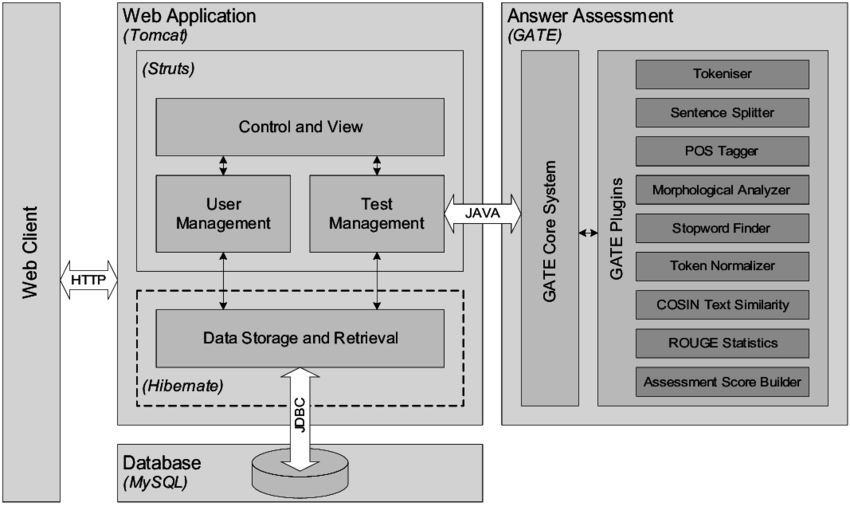
\includegraphics[width=\textwidth]{img/e-examiner}
    \caption{ Architecture of e-Examiner ~\cite{e-examiner}. }\label{fig:e-examiner}
\end{figure}

The system has a user-friendly interface, where user can choose which of the ROUGE techniques should be applied -- see Fig. \ref{fig:e-examiner_Interface}.\\

\begin{figure}[h!]
  \centering
  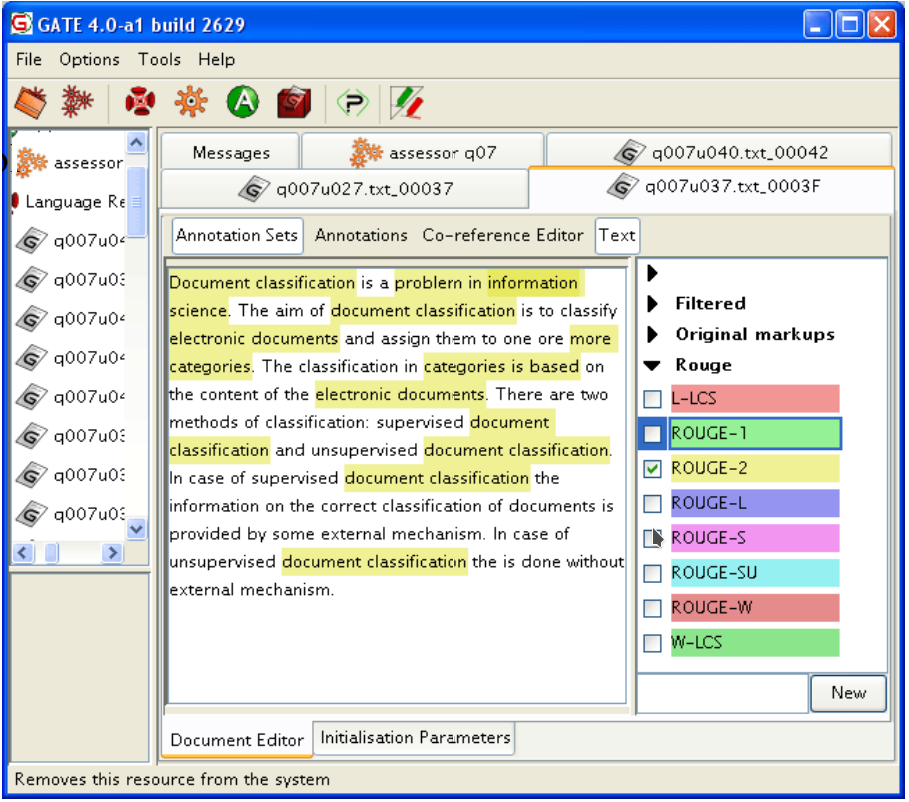
\includegraphics[width=\textwidth]{img/e-examiner_Interface}
    \caption{ Architecture of e-Examiner ~\cite{e-examiner}. }\label{fig:e-examiner_Interface}
\end{figure}

To evaluate the performance of the system datasets from The Institute for Information Systems and New Media (IICM) and Faculty of Engineering, Al-Quds University, Jerusalem were chosen. IICM consists of 5 computer science questions, 5 example answers and 23 sets of students' answers. From the second dataset were taken 3 questions, 3 example answer and also 23 sets of student's answers. The best result -- 81\% -- was achieved using a combination of all ROUGE techniques and cosine similarity.\\

Content Assessment Module (\textbf{CAM}) ~\cite{CAM} is a system for grading of assignments on  English as a Second Language (ESL) test. A dataset for evaluation of the system is taken from this test. It includes 75 questions 566 students' answers, having an example answer is not required. In this method the answers are divided into a graded and test sets and the answers from the test set are compared to the ones from the graded set using a number of NLP techniques: tokenization (breaking a sentence into separate words -- tokens -- and removing punctuation, basically unigrams), lemmatization, spelling correction and noun phrase chunking (NP chunking -- break sentences into subconstituents, i.e. verbs, nouns, and prepositional phrases) -- for preprocessing, and similarity metrics -- for preprocessed text similarity calculation. For these tasks the following tools were used:
\begin{itemize}
\item MontyLingua -- Java/Python NLP toolkit (\url{http://alumni.media.mit.edu/~hugo/montylingua/doc/MontyLingua.html}),
\item PC-KIMMO --  morphological analysis two-level processor  (\url{http://www.ai.mit.edu/courses/6.863/doc/pckimmo.html}),
\item Spell Checker Oriented Word Lists (SCOWL) -- spelling correction for English (\url{https://github.com/en-wl/wordlist}),
\item TreeTagger -- part-of-speech annotation tool for many languages (\url{http://www.cis.uni-muenchen.de/~schmid/tools/TreeTagger/}),
\item CASS -- a tool for chunking (\url{http://spraakdata.gu.se/svedk/cass_swe.html}),
\item WordNet -- considered in "Information extraction methods" section,
\item PMI-IR -- considered in "Corpus-based methods and metric" section,
\item Stanford parser -- a statistical tool for structure of sentences parsing (\url(https://nlp.stanford.edu/software/lex-parser.shtml)).
\end{itemize}


\begin{figure}[h!]
  \centering
  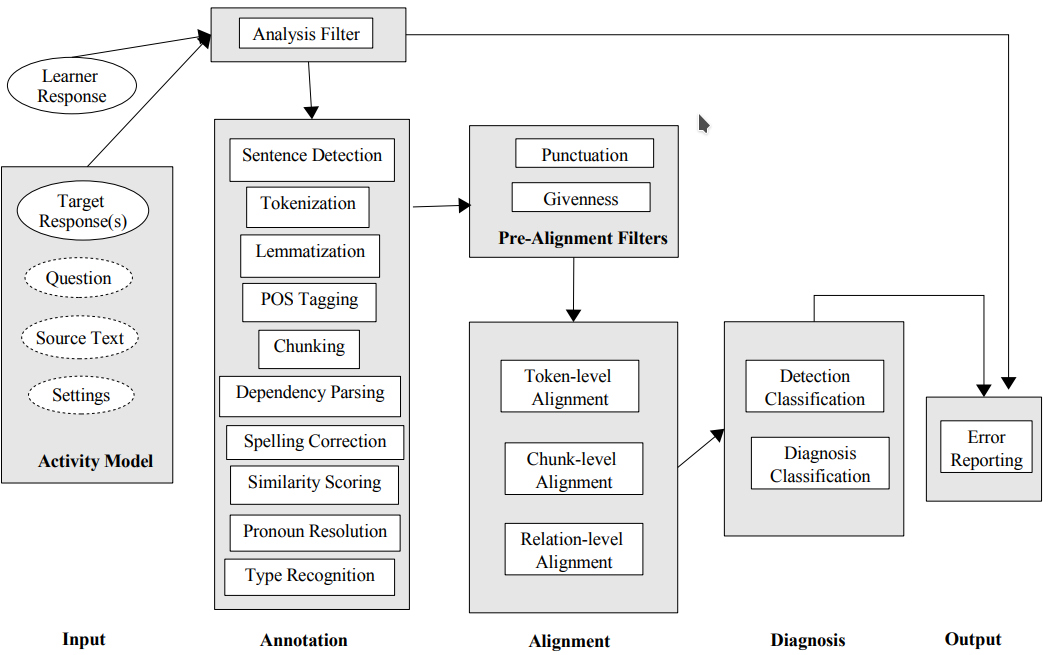
\includegraphics[width=\textwidth]{img/CAM}
    \caption{ Architecture of CAM ~\cite{CAM}. }\label{fig:CAM}
\end{figure}


 The following features were used ~\cite{CAM}:
\begin{itemize}
\item Keyword overlap -- percent of graded-test aligned keywords 
\item Graded and test overlaps -- percents of aligned graded and test tokens 
\item Graded and test chunk -- percents of aligned graded and test chunks
\item Graded and test trigrams -- percent of aligned graded and test trigrams
\item Unigram match -- percent of identical graded and test unigrams
\item Similarity match -- percent of similar tokens
\item Type match -- percent of type-resolved token alignments
\item Lemma match -- percent of lemma-resolved token alignments
\item Synonym match -- percent of synonym-resolved token alignments
\item Variety of match -- number of token-level alignments types
\end{itemize}

These features are used with Tilburg Memory-Based Learner (TiMBL) classifier and thereby reach 88\% of human-computer correlation. TiMBL is based on k-nearest neighbor (KNN) classifier modified in such a way that the nearest neighbors are searched in a decision-tree structure ~\cite{TiMBL}. It is open-source and can be downloaded on the following website: \url{https://languagemachines.github.io/timbl/}. The last commit in TiMBL's github repository (\url{https://github.com/LanguageMachines/timbl}) was on 7th of February 2018, which shows that it is still relevant. \\

Comparing Meaning in Context (\textbf{CoMiC-EN}) ~\cite{CoMiC-EN} and \textbf{CoMiC-DE} ~\cite{CoMiC-DE} are systems for grading reading comprehension assignments in English and German correspondingly. The work is strongly based to CAM approach. It uses the same dataset (for CoMiC-EN) and ML method -- TiMBL. However, there are the following differences:

\begin{itemize}
\item whereas there is only strict unigram-unigram and chunk-chunk comparison in CAM, CoMiC can also compare unigrams with chunks. It is important, because a several words often have a similar meaning to the one word, e.g. "green-eyed monster"-"jealousy".
\item whereas CAM just removes punctuation and words already mentioned in a question from the answers, CoMiC keeps it to save the coherence of the sentence.
\item an updated architecture.  As a basis for its architecture CoMiC employs  Unstructured Information Management Architecture (UIMA), which is an efficient architecture for working with large amounts of unstructured information -- "whose intended meaning is only loosely implied by its form" ~\cite{UIMA}, which is natural language texts, pictures, videos, etc. Structured information would be the one that has a direct relation between the information and form, e.g. a database. UIMA-based architecture of CoMiC is shown in Fig. \ref{fig:UIMA}.

\begin{figure}[h!]
  \centering
  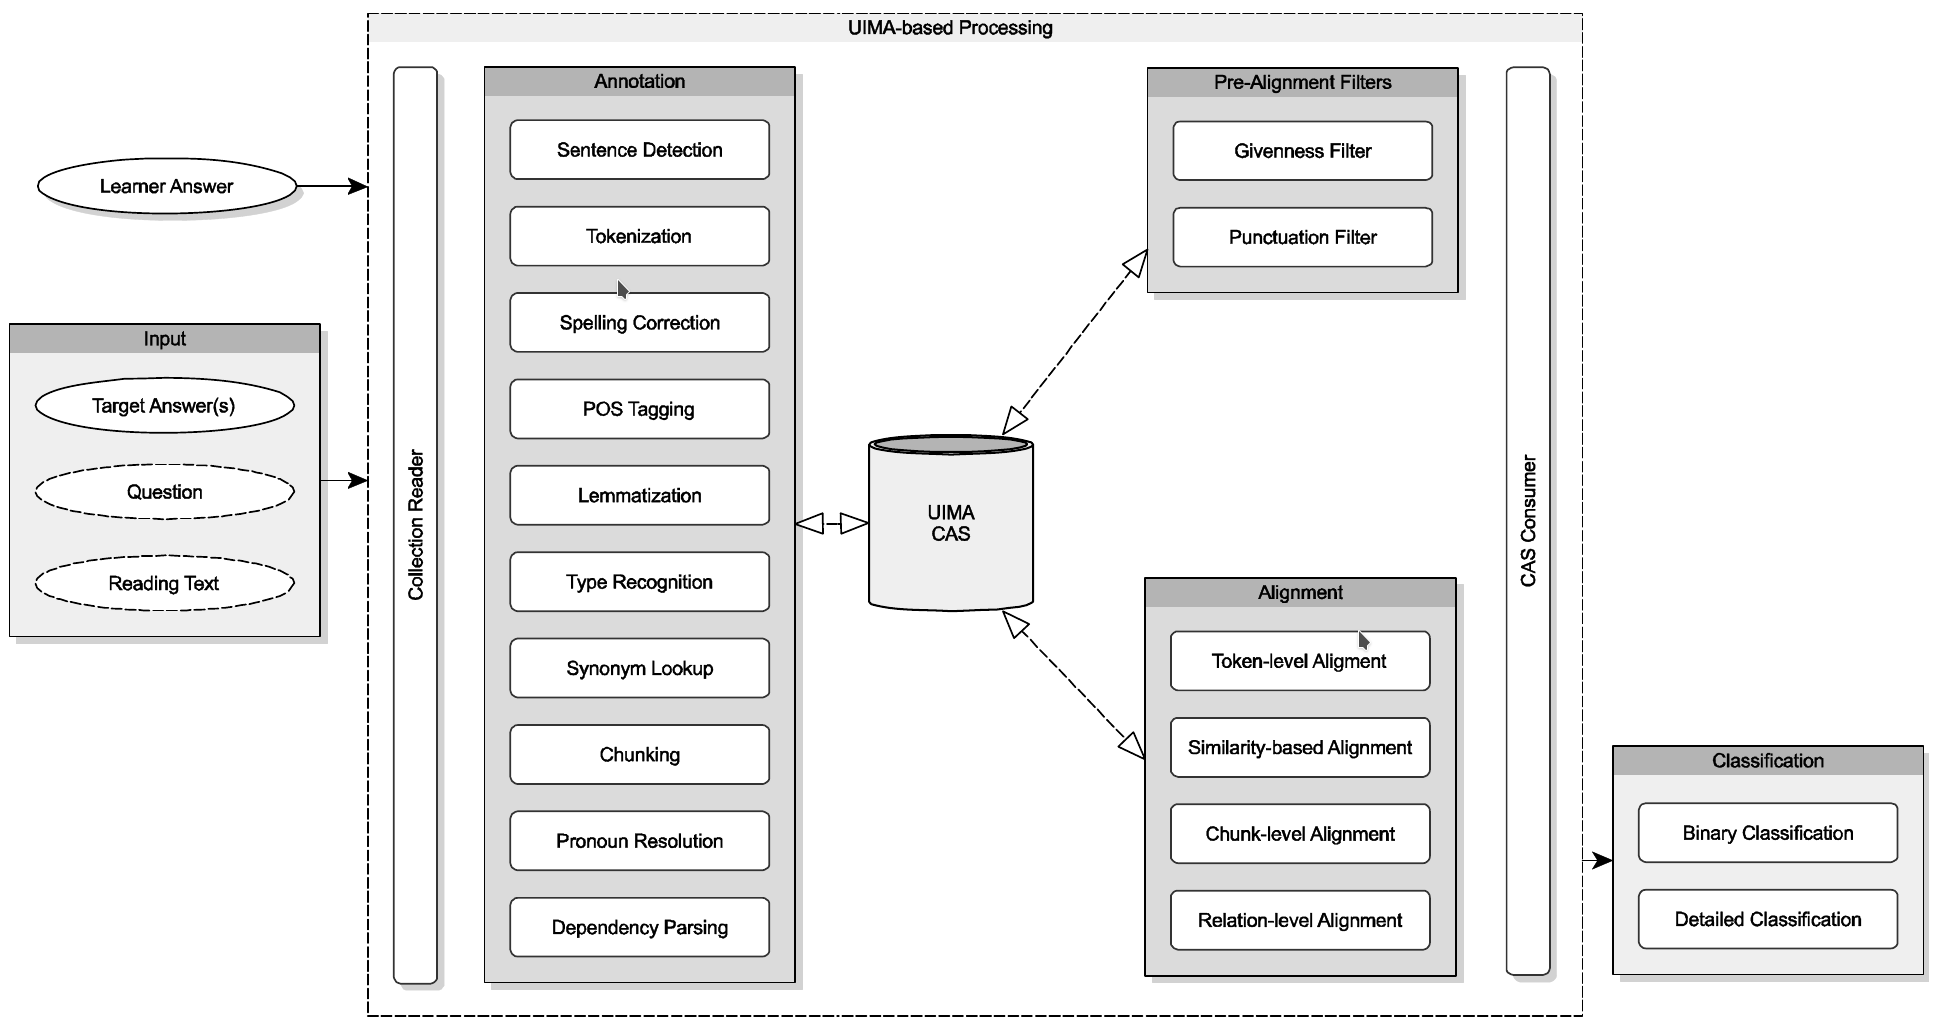
\includegraphics[width=\textwidth]{img/UIMA}
    \caption{ Architecture of CoMiC ~\cite{CoMiC-EN}. }\label{fig:UIMA}
\end{figure}

\item CoMiC uses different NLP tools for their extraction:
\begin{itemize}
\item Apache OpenNLP toolkit (\url{https://opennlp.apache.org/}) instead of MontyLingua and CASS,
\item Morpha -- Java tool for morphological analysis (\url{https://github.com/knowitall/morpha}) instead of PC-KIMMO,
\item MaltParser -- a data-driven dependency parsing (\url{http://www.maltparser.org/}) instead of Stanford parser.
\end{itemize}
The rest of the tools (SCOWL, TreeTagger, WordNet and PMI-IR) remained the same.
\item CoMiC uses the following features: "cosine distance, dot product, weighted overlap, Levenshtein distance, Euclidean distance, modified value difference, Jeffrey divergence and numeric overlap" ~\cite{CoMiC-EN}. All of the have already been described above.
\item CoMiC-EN is not only capable to estimate if the answer was correct or not, bit also provide a detailed information, i.e. which concepts were missing and which were added.
\end{itemize} 

CoMiC shows an insignificantly better result than CAM -- 88.4\% vs 88\%. Nevertheless, the main idea of the paper was to introduce an UIMA architecture and new NLP tools for ASAG. It is also important that CoMiC-EN corpus is available for other researchers, which allows them to compare their results with the ones in the paper. It is not suitable for the current work though, because we focus on computer and natural science.\\

CoMiC-DE is conceptually identical to CoMiC-EN, but focuses on German languag and uses Corpus of Reading comprehension Exercises
in German (CREG). It is the first work that considers automated grading of reading comprehension in German. One can suggest that English and German languages might require slightly different NLP-prepsocessing, however, in this paper the same tools are used and results of English and German ASAG were identical.\\

In \textbf{Zbontar}'s ~\cite{Zbontar} paper a stacking method is used. The main idea of the stacking is combining not only of several metrics, but also of several machine learning methods. The following preprocessing was used: lowercasing, removal of all punctuation, spelling correction, breaking text into 4- and 6-character-grams and creating bag-of-words model based on the n-grams. It is important that character n-grams were used, for usually sentences are broken into word-n-grams. Word-n-grams were already considered before. Character n-grams, e.g. with n = 4, would break a sentence in the following way: "finnegans wake" = \{"finn", "inne", "nneg", "nega", "egan", "gans", "ans ", "ns w", "s wa", " wak", "wake"\}. The following machine learning methods were used: Ridge Regression (RR), SVM -- with lineal and RBF kernels, Gradient Boosting Machine (GBM), Random Forests (RF) and KNN. Different combination of methods were used with different preprocessing:
\begin{itemize}
\item RR, GBM and RF -- with 4-grams
\item RR, SVM-RBF, GMB -- with spelling correction + 4-grams
\item RR, SVM-RBF -- with 6-grams
\item RR, SVM-RBF, KNN -- with spelling correction + 6-grams
\item SVM-RBF -linear, KNN -- with bag-of-word model based on 4-grams + latent semantic indexing with 200 components // TODO: what it is
\item SVM-RBF, GBR, KNN -- with bag-of-word model based on 4-grams + latent semantic indexing with 500 components
\end{itemize}

For evaluation of the method a Kaggle dataset ~\cite{kaggleSas} was used. As Mohler's dataset, this one also contains grades of two human graders. To avoid ambiguity, author just discards the answers graded differently. For the rest of the answers only the grade given by the first human was considered for the learning.

\begin{table}[h!]
\centering
\caption{Machine learning systems}
\label{ML}
\begin{tabular}{|l|l|l|l|}
\hline
System & Year & Approach & Accuracy \\ \hline
e-Examiner & 2007 & \begin{tabular}[x]{@{}c@{}} ROUGE (all) + cosine similarity + \\linear regression \end{tabular} & 81\% \\ \hline
CAM & 2008 &  \begin{tabular}[x]{@{}c@{}} keyword, token, chunk and\\ triple overlaps+\\+ TiMBL-based classifier \end{tabular}  & 88\% \\ \hline
CoMiC-EN/-DE & 2011 &  \begin{tabular}[l]{@{}c@{}} keyword, token, chunk and\\ triple overlaps+\\+ TiMBL-based classifier \end{tabular}  & 88.4\% \\ \hline
Hou & 2011 &  \begin{tabular}[l]{@{}c@{}}   \end{tabular}  &  \% \\ \hline
Zbontar & 2012 & \begin{tabular}[l]{@{}c@{}} bag-of-words of\\character-n-grams\\RR, SVM-RBF,\\GMB, KNN, RF \end{tabular}  &  73.892\% \\ \hline
Horbach & 2013 & \begin{tabular}[l]{@{}c@{}}   \end{tabular}  &  \% \\ \hline
Madnani & 2013 & \begin{tabular}[l]{@{}c@{}}   \end{tabular}  &  \% \\ \hline
SemEval & 2013 &  \begin{tabular}[x]{@{}c@{}} \end{tabular}  & \% \\ \hline
Sultan & 2016 & \begin{tabular}[l]{@{}c@{}}   \end{tabular}  &  \% \\ \hline
Zhang & 2016 & \begin{tabular}[l]{@{}c@{}}   \end{tabular}  &  \% \\ \hline
Pribadi & 2017 & \begin{tabular}[l]{@{}c@{}}   \end{tabular}  &  \% \\ \hline
\end{tabular}
\end{table}


 

\begin{table}[h!]
\centering
\caption{Machine learning systems}
\label{ML}
\begin{tabular}{|l|l|l|l|}
\hline
 System & Year & Features &  Learning algorithm\\ \hline
 CAM & 2008 & \begin{tabular}[x]{@{}c@{}} teacher-student answers \\ overlap \end{tabular} & k-nearest neighbor classifier \\ \hline
 Nielsen '08 & 2008 & \begin{tabular}[l]{@{}c@{}} lexical \\ and syntactic features \end{tabular} & C4.5 decision tree \\ \hline
 CoMiC-EN & 2011 & \begin{tabular}[l]{@{}c@{}} keyword, token, chunk and\\ triple overlaps \end{tabular}  & TiMBL-based classifier\\ \hline
 CoMiC-DE & 2011 & \begin{tabular}[l]{@{}c@{}} keyword, token, chunk and\\ triple overlaps \end{tabular}  & TiMBL-based classifier \\ \hline
 Hou '11 & 2011 & \begin{tabular}[l]{@{}c@{}} POS tags, term frequency,\\ tf.idf, and entropy \end{tabular} & SVM  \\ \hline
 Horbach '13 & 2013 & \begin{tabular}[l]{@{}c@{}} n-gram features + used in \\ CoMiC-EN  \end{tabular}  & k-nearest neighbors \\ \hline
 Madnani '13 & 2013 & \begin{tabular}[l]{@{}c@{}} BLEU, ROUGE, \\number of sentences \end{tabular}  & logistic regression classifier \\ \hline
 Tandella '12 & 2012 & four- and six-grams & \begin{tabular}[l]{@{}c@{}}Stacking of the following:\\ random forests, \\ k-nearest neighbor \\ classifier, SVM, \\ gradient boosting machine, \\ ridge regression)  \end{tabular} \\ \hline
\begin{tabular}[l]{@{}c@{}} Deep Learning \\Student Modeling \\Clustering \end{tabular}  & 2016 & \begin{tabular}[l]{@{}c@{}} text similarity between \\ student and example answer\end{tabular} &  \begin{tabular}[l]{@{}c@{}}  Deep Belief Networks\\ with restricted \\ Boltzmann machine \end{tabular} \\ \hline
\end{tabular}
\end{table}

Deep learning methods were already widely applied to AES, but so far there is only one paper that applies a deep learning approach to ASAG ~\cite{Zhang}. The author proposes usage of deep belief networks (DBN) that uses restricted Boltzmann machine and compares it with classic classifiers such as naive Bayes, logistic regression, decision tree, artificial neutral network and SVM. It was shown that DBN outperforms the other classifiers, except for SVM and SVM is better only in sensitivity. However, the paper focuses mostly on various text similarity measurements, which alone, as mentioned in ~\cite{Sultan}, is not an adequate measure of answer accuracy. \\


\subsubsection{State of the art summary}

"Natural language processing development" section provides a brief overview of a language structure and the general trends of NLP development (Fig. \ref{fig:NLPLevels}). Understanding of linguistic base of NLP helps to see how it is possible to preprocess text in order to improve the process of grading, e.g. by spelling correction, lemmatization and disambiguation. Moreover, it shows the importance of usage of sublanguage that can reduce the amount of words from thousands to several hundreds. Considering various fields of NLP is also important, because ASAG is not a separate scientific discipline -- most or all of the ASAG techniques has already been used in other NLP-fields, for example, BLUE -- for translation and ROUGE -- for evaluation of summaries. It is always important to look for the new methods in various adjacent fields.\\

AES is the most adjacent to ASAG area. The very first AES and ASAG methods were on the opposite sides of automated grading methods: for ASAG it was keyword-spotting, a very specific approach, and for AES it was evaluation of the most general features -- the length of words and sentences. However, in later works one can see how these two areas are moving towards each other and towards understanding of real meaning and style of the text. ASAG and AES share some common methods, like LSA and various metrics, but all of the methods from AES are interesting for ASAG. For example, it is much less than AES vulnerable to gibberish on the word level. \\

AES research started earlier than ASAG and that is why papers on this topic contain some useful general information. The first important idea is the comparison of human graders and computers. The correlation between the human rates was lower -- around 76\% -- than even the very first AES system. ASAG questions are more straightforward, which usually rises the correlation between humans to 80\%-85\%, but it is still far from perfect. That is why 80\%-90\% result for an ASAG system is already satisfying. Moreover, it is not possible to reach 100\% correlation with a human rater, because the human raters simply give different grades.\\

Another important moment is the reason why the first AES system achieved good results. It was trained on rather convenient dataset. The system was vulnerable to any sort of gibberish, but was only trained and tested on a meaningful dataset. It shows that it is always important to test the method on different datasets and, to compare to other works, try to use the same datasets those were used in those works. The importance of datasets one can see also in further ASAG papers, when in the paper that presents the system it achieves 87\% to 94\% ~\cite{c-rater} and, when tested on another dataset by other author, it reaches only 22\% ~\cite{Mohler}. That is why all the accuracies provided in the tables above or below don't provide enough clarity on how good the methods are. However, without testing the each system manually on different kinds of data, it is the only way to compare them at least approximately. The performance of the most significant ASAG systems is shown in Table *ref*.

-- best methods table

Current work focuses on machine learning methods for ASAG and that is why concept or facet mapping and information extraction are considered mostly to complete the picture. However, the corpus-based section was considered in details, because many machine learning approaches often use similarity metrics those were mentioned in the "Corpus-based methods" section. In table \ref{sim} the similarity metrics are summarized. The accuracy column is taken from Noorbehbahani's ~\cite{Noorbehbahani} (marked as "N"), Mohler's ~\cite{Mohler} ("M"), Li's ("L") and Gomaa's ("G") works. It is important not to forget that the accuracy was obtained on different datasets, and therefore the comparison is not entirely valid. Also, Noorbehbahani doesn't mention, which of the ROUGE methods was used, and it is confusing, because in other papers *ref* it performed significantly better. //TODO: add formulas and  Mohler's metrics. Add ROUGE ref\\

\begin{figure}[h!]
  \centering
  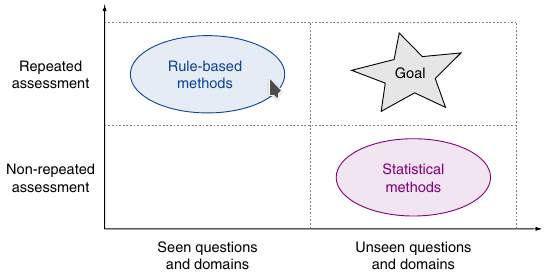
\includegraphics[width=0.7\textwidth]{img/ruleVSstat}
    \caption{  trade-offs between rule-based and statistical methods~\cite{Burrows}. }\label{fig:rVSs}
\end{figure}

Dealing with two human graders -- consider only one -- Zbontar. Discard the discord.

Mostly used languages: Java. Python.\\

Add a list of actually used systems -- the ones with interface and stuff\\

Add a tool table -- word2vec, glove, disco, montilingua, etc.\\

English/German -- the same NLP tools used in CoMiC-EN and -DE. \\

Add list of corpora (wiki \url{https://en.wikipedia.org/wiki/List_of_text_corpora}):
Google Books Ngram Corpus[1][2]
American National Corpus
Bank of English
British National Corpus
Corpus Juris Secundum
Corpus of Contemporary American English (COCA) 425 million words, 1990–2011. Freely searchable online.
Brown Corpus, forming part of the "Brown Family" of corpora, together with LOB, Frown and F-LOB.
International Corpus of English
Oxford English Corpus
Scottish Corpus of Texts \& Speech
Corpus Resource Database (CoRD), more than 80 English language corpora.[3]
RE3D (Relationship and Entity Extraction Evaluation Dataset)

\begin{table}[h!]
\centering
\caption{Similarity metrics}
\label{sim}
\begin{tabular}{|l|l|l|}
\hline
 System & Formula & Accuracy \\ \hline
 ROUGE (N)& 2009 & 22\%  \\ \hline
 BLEU (N)& 2006 & 36\% \\ \hline
 ERB (N)& 2009 & 41\%  \\ \hline
 n-gram co-occurrence (N)& 2006 & 48\% \\ \hline
 LSA & n/a & 51\% (N) or 67.35\% (M) \\ \hline
 LSA \& n-grams (N)&  & 59\%  \\ \hline
 M-BLEU (N)& 2011 & 85\% \\ \hline
\end{tabular}
\end{table}


\chapter{\textbf{Problem formulation}}
In this work we focus on automated short answer grading. 

In general one is concerned neither with writing style nor with spelling or grammar in ASAG. However, we are going to add a feature that would allow the professor who conducts a test to set the strictness of the evaluation: he or she should be able to set if the answers with misspelled words, especially specific terms, should be accepted. The teacher should also be able to estimate how large should be the range of synonyms that the student can use. For example, a professor might not want students to use a word "thing" instead of "entity", though in a certain context from a linguistical point of view it may look as a valid synonym.\\


//Spelling correction is an important aspect of the input
understanding, as students frequently misspell words,
abbreviate creatively, and make word boundary
errors (two words joined together or a single word
split in two). Spelling correction is based on a three-
way match algorithm which slides a small window
simultaneously across both the unknown input word
and a candidate word from the lexicon.
Transpositions, elisions, substitutions, and similar
errors are counted and the most likely candidate is
picked.(Evens, M.W., Zhang, Y., Michael, J.A., \& Rovick, A.A.
(1997). CIRCSIM-Tutor: An Intelligent Tutoring System
Using Natural Language Dialogue. Morgan Kaufmann
Publishers, 13-14.)// 

As for the result of the grading, it is important to provide not only the grade, but a level of certainty of the grading and in the perfect case -- generate the comments to each graded answer. For the comment generating we will need an additional set of teachers' comments corresponding to the answers. \\

Another side of the problem is a small amount of data that we posess now. Moreover, this data should be also carefully examined, because the ASAG questions can be formulated in improper way. The questions must meet certain criteria ~\cite{Hasanah}:
\begin{itemize}
\item The question must not contain any information that can let a student to obtain the answer from the question, i.e. the student must be able to formulate the answer based only on his or her external knowledge;
\item In general the question must require a strictly natural language answer. Current work focuses on the natural language part. However, in our project we are going to allow a combination of natural language, formulas, pictures and programming code.
\item The question must be formulated in such a way that student could give an answer between one sentence and one paragraph length.
\item The question must be formulated in the least ambiguous way to increase the level of close-ended responses.
\end{itemize}


\section*{\textbf{Software overview}}
\subsection{Software for e-assessments}

Before introducing a new system it is crucial to consider the existing ones. Since the autograding system will be tested in Hochschule Bonn-Rhein-Sieg first, we need to consider the question and answer types provided in the testing system of LEA -- see Table \ref{lea}.

// add a table with other systems used in different schools

Question types: \url{https://lea.hochschule-bonn-rhein-sieg.de/goto.php?target=wiki\_360501\_Welche\_Fragentypen\_gibt\_es\_und\_was\_mache\_ich\_damit\%3F}
\begin{table}[]
\centering
\caption{LEA question types}
\label{lea}
\begin{tabular}{|l|l|l|}
\hline
Single Choice Frage	
 & Eine der vorgegebenen Antworten auswählbar & Autograded \\ \hline
 Multiple Choice Frage & Frage	
Mehrere der vorgegebenen Antworten auswaehlbar & Autograded \\ \hline
 Kprim Choice & 	
Vierfachauswahl "richtig/falsch" & Autograded\\ \hline
 Fehler/Worte markieren & Fehler in vorgegebenem Text markieren & Autograded\\ \hline
 Hotspot/ImageMap-Frage & Richtige Stellen in anklickbarem Bild anklicken & Autograded\\ \hline
 Lückentextfrage & 	
Antworten in Lückentext eingeben & Autograded\\ \hline
 Numerische Antwort & Eingabe einer Zahl & Autograded\\ \hline
 Formelfrage (only numbers)	
 & Rechenaufgabe
(Formel mit Variablen werden vorgegeben, Zahlenwerte werden zufällig aus definierten Zahlenräumen gewählt) & Autograded\\ \hline
 Begriffe benennen & 	
Auflistung geforderter Begriffe & Autograded\\ \hline
 Anordnungsfrage  & Reihenfolge vorgegebener Antworten in vertikaler Anordnung anpassen & Autograded\\ \hline
 Zuordnungsfrage & Elemente einer Teilmenge(Eigenschaften) einem Begriff (Definitionen) zuordnen & Autograded\\ \hline
 Freitext eingeben & Textantwort & Autograded\\ \hline
 Datei hochladen & Antwort in Dateiform hochladbar & Autograded\\ \hline
 Eingebettete Frage: Flash & Frage/Antwort mittels Flash-Objekt einbinden & Autograded\\ \hline
 Eingebettete Frage: Java Applet & Frage/Antwort mittels Java-Applet einbinden & Autograded\\ \hline
\end{tabular}
\end{table}
 insert pictures with example of questions
 write about the interface, 1 question at a time and all this
 
\subsection{GUI and grading: Jupyter and Nbgrader}

\subsection{Software for ASAG}




\chapter*{\textbf{Our approach}}

// feature -- answer length: "A
candidate's lack of knowledge can lead to answers that are
difficult to comprehend, and excessively lengthy answers can mask this lack of knowledge. " ~\cite{Thomas}
...

\section{Architecture}

draw an architecture similar to Willow's

\section{Dataset description}

\section*{English vs German}

\begin{itemize}
\item More word forms -> lemmization
\item Separable prefixes. words like "davon"
\item verb position in different subordinate clauses
\item less fixed non-verb word order -- one can easily exchange word positions to emphasize some idea
\end{itemize}

\section*{Kernel Principal Component Analysis (KPCA)}

//write more about N-grams and distance evaluation in one of the previous parts 

N-grams representation allows a simple calculation of the distance between long sentences. It is not much more complex than a simple keywords approach, but allows to take into consideration sequences of the words, which is important for avoidance of senseless word order similar to the one in the following example  ~\cite{cover}: "A complex pattern-classification problem, cast in a \textbf{low-dimensional} space nonlinearly, is more likely to be linearly separable than in a \textbf{high-dimensional}, provided that the space is not densely populated.". Here words "low-dimensional" and "high-dimensional" are exchanged and a perfectly correct from the keywords point of view formulation of Cover's theorem becomes completely wrong. However, n-gram analysis can help to avoid it, because it is looking not only for "low-dimensional", but for n-grams like "cast in a high-dimensional" and "than in a low-dimensional", so  "cast in a low-dimensional" and "than in a high-dimensional" are incorrect.\\

N-gram distance solely is not enough to create a sensible feature for the machine learning. It requires further preprocessing. ~\cite{eduardo} describes KPCA for word embedding based on n-gram similarity, where n-grams are sequences of the letters inside the word. In combination with k-means this algorithm was shown to be more effective for german verbs classification ~\cite{eduardo} than word2vec ~\cite{word2vec}, because word2vec doesn't take into account morphological structure of the words. That is why this method was chosen to be extended in such a way that it will be accepting sentences and calculate distances between n-grams those are words sequences.\\

The idea of the KPCA is mapping of data vectors to the feature space for principal component extraction. It is quite similar to the regular PCA, but the inner product in the feature space is computed using a kernel function, which is usually RBF or polynomial. The following derivation is based on ~\cite{eduardo} and  ~\cite{readingGroup}. To perform KPCA one should take the m-dimensional data matrix: $\pmb{X} = [\pmb{x_1}, \pmb{x_2}, ..., \pmb{x_n}]$ and start with PCA representation:

\begin{equation} \label{eq:1}
\pmb{Cv}=\lambda \pmb{v},
\end{equation}

where $\pmb{C} = \frac{1}{n}\pmb{XX^T}$ -- covariance matrix of  $\pmb{X}$, $\lambda$ and $\pmb{v}$ -- eigenvalue and corresponding eigenvector. That is why \ref{eq:1} can be rewritten in the following way:

\begin{equation} \label{eq:2}
\frac{1}{n\lambda}\pmb{XX^T}\pmb{v} = \pmb{X\alpha} = \pmb{v},
\end{equation}

where $\pmb{\alpha} \in R^m$ and it will play a role of an eigenvector for kernalized PCA:

\begin{equation} \label{eq:3}
\pmb{XXX^T}\pmb{v} = n\lambda \pmb{X\alpha},
\end{equation}

adding $\pmb{X^T}$ from the left:

\begin{equation} \label{eq:4}
\pmb{X^TXXX^T}\pmb{v} = n\lambda \pmb{X^TX\alpha},
\end{equation}

$ \pmb{X^TX}$ would be the kernel matrix $\pmb{K}$ and $n\lambda$ = $\widetilde{\lambda}$, which would be the new eigenvalue:

\begin{equation} \label{eq:5}
\pmb{KK}\pmb{v} = \widetilde{\lambda} \pmb{K\alpha},
\end{equation}

dividing both parts by $\pmb{K}$ we obtain the final form of KPCA equation:

\begin{equation} \label{eq:6}
\pmb{K}\pmb{v} = \widetilde{\lambda} \pmb{\alpha},
\end{equation}

Kernel matrix $\pmb{K}$ is obtained by applying a kernel function to similarity matrix $\pmb{S}$, which is calculated by evaluating similarity between each pair of data elements (words, sentences, etc.) in the given dataset. In our case it is based on  S{\o}rensen-Dice or Jaccard distances between the n-grams in sentences.\\

// add "bag of n-grams"

//write more about the distances after reading more

Problem with German: "some morphologically rich languages \ref{eq:1}
(where these models are supposed to perform specially well) may contain very
long words. This leads to a dramatic increase of the number of necessary n-gram
representations, increasing time and space complexity as well."


Method: page with formulas from Eduardo's paper

compare it to word2vec


\begin{thebibliography}{3}
\bibitem{Hasanah} U. Hasanah, A. E. Permanasari, S. S. Kusumawardani and F. S. Pribadi, "A review of an information extraction technique approach for automatic short answer grading," 2016 1st International Conference on Information Technology, Information Systems and Electrical Engineering (ICITISEE), Yogyakarta, 2016, pp. 192-196.
\bibitem{Burrows} Burrows S., Gurevych I., Stein B. The eras and trends of automatic short answer grading //International Journal of Artificial Intelligence in Education. -- 2015. -- T. 25. -- No. 1. -- C. 60-117.
\bibitem{Balfour} Balfour, S. P. (2013). Assessing writing in MOOCS: Automated essay scoring and Calibrated Peer Review. Research \& Practice in Assessment, 8(1), 40--48.
\bibitem{aesOverview} S. Dikli  An overview of automated scoring of essays //The Journal of Technology, Learning and Assessment. -- 2006. -- T. 5.-- No. 1.
\bibitem{vikGit} \url{https://github.com/VikParuchuri/vikparuchuri-affirm/blob/master/on-the-automated-scoring-of-essays.md}
\bibitem{HewlettKaggle} \url{https://www.kaggle.com/c/asap-aes/discussion}
\bibitem{edxGit} \url{https://github.com/edx/ease}
\bibitem{Shermis} M. Shermis and B. Hammer. 2012. Contrasting state-of-the-art automated scoring of essays: analysis. Technical report, The University of Akron and Kaggle
\bibitem{Alikaniotis} Alikaniotis D., Yannakoudakis H., Rei M. Automatic text scoring using neural networks //arXiv preprint arXiv:1606.04289. – 2016.
\bibitem{petition} \url{http://humanreaders.org/petition/index.php}
\bibitem{Perelman} Perelman, Les. "Critique of Mark D. Shermis \& Ben Hamner,"Contrasting state-of-the-art automated scoring of essays: analysis"." Journal of Writing Assessment 6.1 (2013).
\bibitem{Byrne} Byrne, Roxanne, Tang, Michael, Truduc, John \& Tang, Matthew. (2010). eGrader, a software application that automatically scores student essays: with a postscript on the ethical complexities. Journal of Systemics, Cybernetics \& Informatics, 8(6), 30-35.
\bibitem{Ramineni} Ramineni, Chaitanya, and David M. Williamson. "Automated essay scoring: Psychometric guidelines and practices." Assessing Writing 18.1 (2013): 25-39. 
\bibitem{Cambria} E. Cambria and B. White, "Jumping NLP Curves: A Review of Natural Language Processing Research [Review Article]," in IEEE Computational Intelligence Magazine, vol. 9, no. 2, pp. 48-57, May 2014.
\bibitem{Page}  Page, E. B. (1966). "The Imminence of Grading Essays by Computer" Phi Delta Kappan, 47(5), 238-243.
\bibitem{Chowdhury} Chowdhury, Gobinda G. "Natural language processing." Annual review of information science and technology 37.1 (2003): 51-89
\bibitem{Steedman} Steedman, Mark. "Natural language processing." Handbook of perception and cognition (2nd ed.). Artificial intelligence (1996): 229-266.
\bibitem{Saad} Ahmad, Saad. "Tutorial on Natural Language Processing." Artificial Intelligence 810.161 (2007).
\bibitem{Raskin}  Raskin, Victor. "Linguistics and natural language processing." Machine Translation: Theoretical and Methodological Issues. Cambridge University Press, Cambridge (1987): 42-58.
\bibitem{Faust} Von Goethe, Johann Wolfgang, "Faust", January 4, 2005 [EBook \#14591], \url{http://www.gutenberg.org/files/14591/14591-h/14591-h.htm}
\bibitem{Blood} Blood, Ian. "Automated essay scoring: a literature review." Teachers College, Columbia University Working Papers in TESOL \& Applied Linguistics 11.2 (2012): 40-64.
\bibitem{Hearst} Marti A. Hearst, ``The debate on automated essay grading'' (http://www.knowledge-technologies.com/presskit/KAT\_IEEEdebate.pdf) 
\bibitem{LSA} Landauer, Thomas K., Peter W. Foltz, and Darrell Laham. "An introduction to latent semantic analysis." Discourse processes 25.2-3 (1998): 259-284.
\bibitem{Dzikovska} Dzikovska, M. O., Nielsen, R. D., Brew, C., Leacock, C., Giampiccolo, D., Bentivogli, L., Clark, P., Dagan, I., and Dang, H. T. (2013). SemEval-2013 Task 7: The Joint Student Response Analysis and Eighth Recognizing Textual Entailment Challenge. In M. Diab, T. Baldwin, and M. Baroni, editors, Proceedings of the Second Joint Conference on Lexical and Computational Semantics, pages 1-12, Atlanta, Georgia.
\bibitem{c-rater}  Leacock, Claudia, and Martin Chodorow. "C-rater: Automated scoring of short-answer questions." Computers and the Humanities 37.4 (2003): 389-405.
\bibitem{Wang} Wang, Hao-Chuan, Chun-Yen Chang, and Tsai-Yen Li. "Assessing creative problem-solving with automated text grading." Computers \& Education 51.4 (2008): 1450-1466.
\bibitem{Pulman} Stephen G. Pulman and Jana Z. Sukkarieh. 2005. Automatic short answer marking. In Proceedings of the second workshop on Building Educational Applications Using NLP (EdAppsNLP 05). Association for Computational Linguistics, Stroudsburg, PA, USA, 9-16.
\bibitem{Thomas} Pete Thomas. 2003. The evaluation of electronic marking of examinations. In Proceedings of the 8th annual conference on Innovation and technology in computer science education (ITiCSE '03), David Finkel (Ed.). ACM, New York, NY, USA, 50-54. DOI=http://dx.doi.org/10.1145/961511.961528
\bibitem{CREG} \url{https://github.com/carolscarton/CREG-MT-eval}
\bibitem{Hahn} Hahn, Michael, and Detmar Meurers. "Evaluating the meaning of answers to reading comprehension questions a semantics-based approach." Proceedings of the Seventh Workshop on Building Educational Applications Using NLP. Association for Computational Linguistics, 2012.
\bibitem{ERB} Pérez, Diana, Alfio Gliozzo, and Carlo Strapparava. "Automatic Assessment of Students’ free-text Answers underpinned by the Combination of a BLEU-inspired algorithm and Latent Semantic Analysis." (2005).
\bibitem{BLEU} Kishore Papineni, Salim Roukos, Todd Ward, and Wei-Jing Zhu. 2002. BLEU: a method for automatic evaluation of machine translation. In Proceedings of the 40th Annual Meeting on Association for Computational Linguistics (ACL '02). Association for Computational Linguistics, Stroudsburg, PA, USA, 311-318. DOI: https://doi.org/10.3115/1073083.1073135
\bibitem{Willow} Pérez-Marín, Diana, and Ismael Pascual-Nieto. "Willow: a system to automatically assess students’ free-text answers by using a combination of shallow NLP techniques." International Journal of Continuing Engineering Education and Life Long Learning 21.2-3 (2011): 155-169.
\bibitem{SAMText} Bukai, Ohad Lisral, Robert Pokorny, and Jacqueline A. Haynes. "Automated short free-text scoring method and system." U.S. Patent Application No. 11/895,267.
\bibitem{Mohler} Mohler, Michael, and Rada Mihalcea. "Text-to-text semantic similarity for automatic short answer grading." Proceedings of the 12th Conference of the European Chapter of the Association for Computational Linguistics. Association for Computational Linguistics, 2009.
\bibitem{Gabrilovich} E. Gabrilovich and S. Markovitch. 2006. Overcoming the brittleness bottleneck using Wikipedia: Enhancing text categorization with encyclopedic knowledge. In Proceedings of the National Conference on Artificial Intelligence (AAAI), Boston.
\bibitem{Klein} R. Klein, A. Kyrilov, and M. Tokman. 2011. Automated assessment of short free-text responses in computer science using latent semantic analysis. In Proceedings of the 16th annual joint conference on Innovation and technology in computer science education (ITiCSE '11). ACM, New York, NY, USA, 158-162. 
\bibitem{Noorbehbahani} Noorbehbahani, Fakhroddin, and Ahmad A. Kardan. "The automatic assessment of free text answers using a modified BLEU algorithm." Computers \& Education 56.2 (2011): 337-345.
\bibitem{Skip-gram} Guthrie, David, et al. "A closer look at skip-gram modelling." Proceedings of the 5th international Conference on Language Resources and Evaluation (LREC-2006). sn, 2006.
\bibitem{Ulysses} Joyce, J. (1969). Ulysses. London: Bodley Head.
\bibitem{Li} Yanling Li and Yonghong Yan, "New similarity measures for automatic short answer scoring in spontaneous non-native speech," International Conference on Automatic Control and Artificial Intelligence (ACAI 2012), Xiamen, 2012, pp. 1398-1402.
\bibitem{Gomaa} Gomaa, Wael H., and Aly A. Fahmy. "Short answer grading using string similarity and corpus-based similarity." International Journal of Advanced Computer Science and Applications (IJACSA) 3.11 (2012).
\bibitem{Jaro} \url{https://rosettacode.org/wiki/Jaro_distance}
\bibitem{DISCO} \url{http://www.linguatools.de/disco/disco_en.html}
\bibitem{word2vec} \url{https://code.google.com/archive/p/word2vec/}
\bibitem{GloVe} Pennington, Jeffrey, Richard Socher, and Christopher Manning. "Glove: Global vectors for word representation." Proceedings of the 2014 conference on empirical methods in natural language processing (EMNLP). 2014.
\bibitem{e-examiner} Guetl, Christian. (2008). Moving towards a Fully Automatic Knowledge Assessment Tool. International Journal of Emerging Technologies in Learning. 3. 
\bibitem{CAM} Bailey, S. \& D. Meurers (2008). Diagnosing meaning errors in short answers to reading comprehension questions. In J. Tetreault, J. Burstein \& R. D. Felice (eds.), Proceedings of the 3rd Workshop on Innovative Use of NLP for Building Educational Applications (BEA-3) at ACL'08. Columbus, Ohio, pp. 107-115.
\bibitem{TiMBL} Daelemans, Walter, et al. "Timbl: Tilburg memory-based learner." version 6 (2007): 07-03.
\bibitem{CoMiC-EN} Meurers, Detmar, et al. "Integrating parallel analysis modules to evaluate the meaning of answers to reading comprehension questions." International Journal of Continuing Engineering Education and Life Long Learning 21.4 (2011): 355-369.
\bibitem{CoMiC-DE} Meurers, Detmar, et al. "Evaluating answers to reading comprehension questions in context: Results for German and the role of information structure." Proceedings of the TextInfer 2011 Workshop on Textual Entailment. Association for Computational Linguistics, 2011.
\bibitem{UIMA} Ferrucci, David, and Adam Lally. "UIMA: an architectural approach to unstructured information processing in the corporate research environment." Natural Language Engineering 10.3-4 (2004): 327-348.
\bibitem{Zbontar} Zbontar, J. "Short Answer Scoring by Stacking" ASAP'12 SAS methodology paper (2012).
\bibitem{kaggleSas} \url{https://www.kaggle.com/c/asap-sas}



\bibitem{Horbach} Horbach, Andrea, Alexis Palmer, and Manfred Pinkal. "Using the text to evaluate short answers for reading comprehension exercises." * SEM@ NAACL-HLT. 2013.
\bibitem{Zhang} Zhang, Yuan, Rajat Shah, and Min Chi. "Deep Learning+ Student Modeling+ Clustering: a Recipe for Effective Automatic Short Answer Grading." EDM. 2016.
\bibitem{Sultan} Sultan, Md Arafat, Cristobal Salazar, and Tamara Sumner. "Fast and easy short answer grading with high accuracy." Proceedings of NAACL-HLT. 2016

\bibitem{Ziai} Ziai, Ramon, Niels Ott, and Detmar Meurers. "Short answer assessment: Establishing links between research strands." Proceedings of the Seventh Workshop on Building Educational Applications Using NLP. Association for Computational Linguistics, 2012.
\bibitem{Roy} Roy, Shourya, Himanshu S. Bhatt, and Y. Narahari. "An Iterative Transfer Learning Based Ensemble Technique for Automatic Short Answer Grading." arXiv preprint arXiv:1609.04909 (2016).
\bibitem{Yin} Yin, Wenpeng, et al. "Comparative Study of CNN and RNN for Natural Language Processing." arXiv preprint arXiv:1702.01923 (2017).
\bibitem{Zanzotto} Zanzotto, Fabio Massimo, Marco Pennacchiotti, and Alessandro Moschitti. "A machine learning approach to textual entailment recognition." Natural Language Engineering 15.4 (2009): 551-582
\bibitem{ipython} \url{https://ipython.org/notebook.html}
\bibitem{nbgrader} \url{https://github.com/jupyter/nbgrader}


\bibitem{eduardo} Brito, Eduardo \& Sifa, Rafet \& Bauckhage, Christian. (2017). KPCA Embeddings: an Unsupervised Approach to Learn Vector Representations of Finite Domain Sequences.
\bibitem{cover} Cover, T.M., Geometrical and Statistical properties of systems of linear inequalities with applications in pattern recognition, 1965 (hghlighted words are exchanged)
\bibitem{readingGroup} \url{https://www.researchgate.net/project/reading-group-machine-learning-AI}


\end{thebibliography}


\end{document}